%!TEX TS-program = pdflatexmk
\documentclass[cleanfoot]{asme2ej}

\usepackage[]{graphicx}
\graphicspath{ {images/} }

\usepackage{enumitem}
\usepackage{amsmath,amssymb}
\usepackage{textcomp}
\usepackage[urlcolor=blue,linkcolor=red,colorlinks=true]{hyperref}
\usepackage[autostyle, english=american]{csquotes}
\MakeOuterQuote{"}

\title{Exoplanet Open-Source Imaging Mission Simulator (EXOSIMS) \\ Interface Control Document}

%%% first author
\author{Daniel Garrett, Christian Delacroix, and Dmitry Savransky
    \affiliation{
    Sibley School of Mechanical and Aerospace Engineering\\
	Cornell University\\
	Ithaca, NY 14853
    }	
}

\def\mf{\mathbf}
\def\mb{\mathbb}
\def\mc{\mathcal}
\newcommand{\R}{\mathbf{r}}
\newcommand{\bc}{\mathbf{b}}
\newcommand{\mfbar}[1]{\mf{\bar{#1}}}
\newcommand{\mfhat}[1]{\mf{\hat{#1}}}
\newcommand{\bmu}{\boldsymbol{\mu}}
\newcommand{\blam}{\boldsymbol{\Lambda}}
\newcommand{\refeq}[1]{Equation  (\ref{#1})} 
\newcommand{\reftable}[1]{Table \ref{#1}} 
\newcommand{\refch}[1]{Chapter  \ref{#1}} 
\newcommand{\reffig}[1]{Figure \ref{#1}}
\newcommand{\refcode}[1]{Listing \ref{#1}}
\newcommand{\intd}[1]{\ensuremath{\,\mathrm{d}#1}}
\newcommand{\leftexp}[2]{{\vphantom{#2}}^{#1}\!{#2}}
\newcommand{\leftsub}[2]{{\vphantom{#2}}_{#1}\!{#2}}
\newcommand{\fddt}[1]{\ensuremath{\leftexp{\mathcal{#1}}{\frac{\mathrm{d}}{\mathrm{d}t}}}}
\newcommand{\fdddt}[1]{\ensuremath{\leftexp{\mathcal{#1}}{\frac{\mathrm{d}^2}{\mathrm{d}t^2}}}}
\newcommand{\omegarot}[2]{\ensuremath{\leftexp{\mathcal{#1}}{\boldsymbol{\omega}}^{\mathcal{#2}}}}


\begin{document}

\maketitle    

%%%%%%%%%%%%%%%%%%%%%%%%%%%%%%%%%%%%%%%%%%%%%%%%%%%%%%%%%%%%%%%%%%%%%%
\begin{abstract}
{\it This document describes the extensible, modular, open source software framework EXOSIMS.  EXOSIMS creates end-to-end simulations of space-based exoplanet imaging missions using stand-alone software modules.  The input/output interfaces of each module and interactions of modules with each other are presented to give guidance on mission specific modifications to the EXOSIMS framework. Last Update: \today}
\end{abstract}

\tableofcontents

%%%%%%%%%%%%%%%%%%%%%%%%%%%%%%%%%%%%%%%%%%%%%%%%%%%%%%%%%%%%%%%%%%%%%%
\begin{nomenclature}
\entry{EXOSIMS}{Exoplanet Open-Source Imaging Mission Simulator}
\entry{ICD}{Interface Control Document}
\entry{MJD}{Modified Julian Day}
\end{nomenclature}

%%%%%%%%%%%%%%%%%%%%%%%%%%%%%%%%%%%%%%%%%%%%%%%%%%%%%%%%%%%%%%%%%%%%%%
% INTRODUCTION
%%%%%%%%%%%%%%%%%%%%%%%%%%%%%%%%%%%%%%%%%%%%%%%%%%%%%%%%%%%%%%%%%%%%%%

\section{Introduction} 
Building confidence in a mission concept's ability to achieve its science goals is always desirable.  Unfortunately, accurately modeling the science yield of an exoplanet imager can be almost as complicated as designing the mission.  It is challenging to compare science simulation results and systematically test the effects of changing one aspect of the instrument or mission design.

EXOSIMS (Exoplanet Open-Source Imaging Mission Simulator) addresses this problem by generating ensembles of mission simulations for exoplanet direct imaging missions to estimate science yields. It is designed to allow systematic exploration of exoplanet imaging mission science yields.  It consists of stand-alone modules written in Python which may be modified without requiring modifications to other portions of the code. This allows EXOSIMS to be easily used to investigate new designs for instruments, observatories, or overall mission designs independently. This document describes the required input/output interfaces for the stand-alone modules to enable this flexibility.

\subsection{Purpose and Scope} % Rework this section
This Interface Control Document (ICD) provides an overview of the software framework of EXOSIMS and some details on its component parts.  As the software is intended to be highly reconfigurable, operational aspects of the code are emphasized over implementational details.  Specific examples are taken from the coronagraphic instrument under development for WFIRST-AFTA.  The data inputs and outputs of each module are described. Following these guidelines will allow the code to be updated to accommodate new mission designs.

This ICD defines the input/output of each module and the interfaces between modules of the code.  This document is intended to guide mission planners and instrument designers in the development of specific modules for new mission designs.

%\subsection{Glossary}
%This section will contain definition of terms used throughout the document if needed.

\section{Overview}
The terminology used to describe the software implementation is loosely based upon object-oriented programing (OOP) terminology, as implemented by the Python language, in which EXOSIMS is built.  The term module can refer to the object class prototype representing the abstracted functionality of one piece of the software, an implementation of this object class which inherits the attributes and methods of the prototype, or an instance of this class.  Input/output definitions of modules refer to the class prototype.  Implemented modules refer to the inherited class definition.  Passing modules (or their outputs) means the instantiation of the inherited object class being used in a given simulation.  Relying on strict inheritance for all implemented module classes provides an automated error and consistency-checking mechanism.  The outputs of a given object instance may be compared to the outputs of the prototype.  It is trivial to pre-check whether a given module implementation will work within the larger framework, and this approach allows for flexibility and adaptability.

% \begin{figure}[ht]
%     \begin{center}
%         \begin{tabular}{c}
%              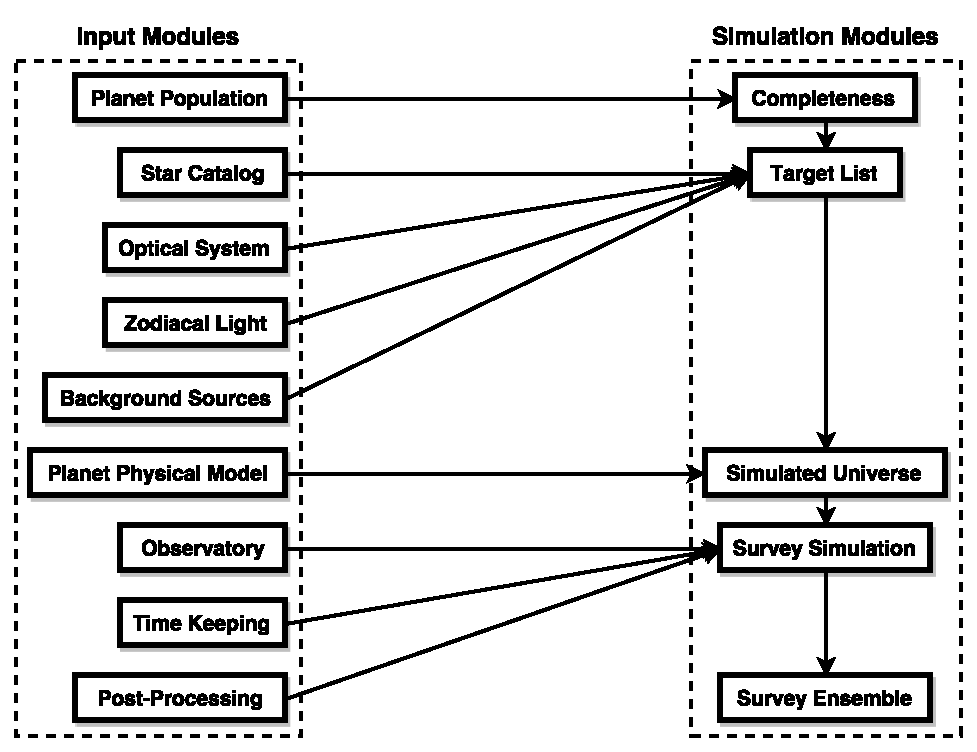
\includegraphics[width=0.9\textwidth]{codeflow5}
%         \end{tabular}
%     \end{center}
%     \caption{EXOSIMS modules. Each box represents a component software module that interacts with other modules as indicated by the arrows. The simulation modules pass all input modules along with their own output.  Thus, the Survey Ensemble module has access to all of the input modules and all of the upstream simulation modules.}
%     \label{figure_framework}
% \end{figure}

The overall framework of EXOSIMS is depicted in \reffig{fig:instantiation_tree} which shows all of the component software modules in the order in which they are instantiated in normal operation. The modules include the Optical System, Star Catalog, Planet Population, Observatory, Planet Physical Model, Time Keeping, Zodiacal Light, Background Sources, and Post-Processing modules and Target List, Simulated Universe, Survey Simulation, and Survey Ensemble modules.  Objects of all module classes can be instantiated independently, although most modules require the instantiation of other modules during their construction. Different implementations of the modules contain specific mission design parameters and physical descriptions of the universe, and will change according to mission and planet population of interest.  The upstream modules (including Target List, Simulated Universe, Survey Simulation, and Survey Ensemble modules) take information contained in the downstream modules and perform mission simulation tasks. The instantiation of an object of any of these modules requires the instantiation of one or more downstream module objects.  Any module may perform any number or kind of calculations using any or all of the input parameters provided.  The specific implementations are only constrained by their input and output specification contained in this document.
\begin{figure}[ht]
    \begin{center}
        \begin{tabular}{c}
             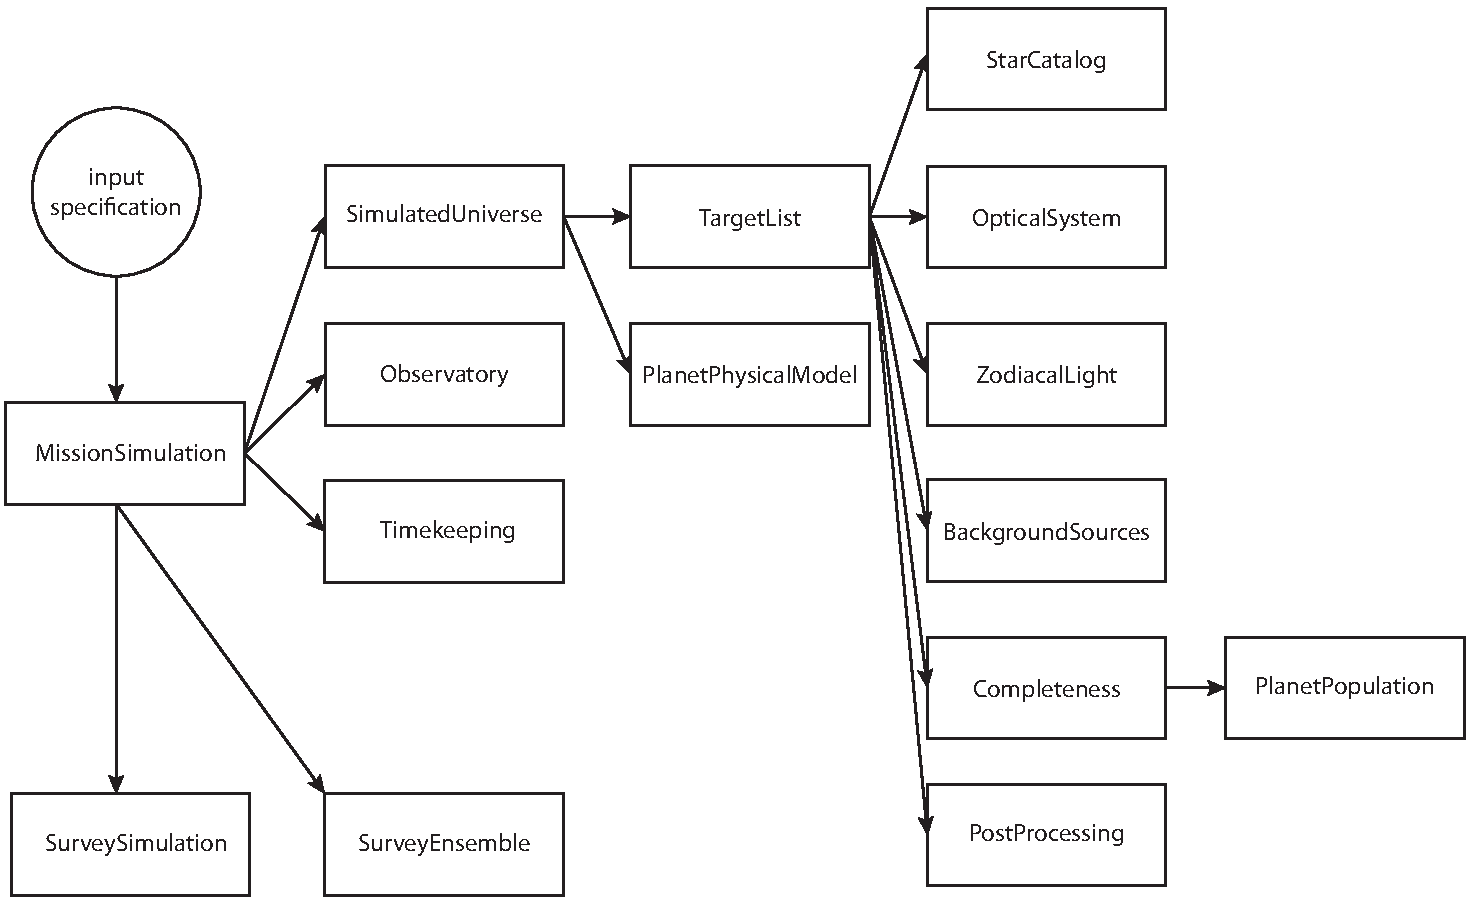
\includegraphics[width=1\textwidth]{instantiation_tree}
        \end{tabular}
    \end{center}
    \caption{Schematic depiction of the instantiation path of all EXOSIMS modules.  The entry point to the backbone is the construction of a MissionSimulation object, which causes the instantiation of all other module objects.  All objects are instantiated in the order shown here, with SurveySimulation and SurveyEnsemble constructed last.  The arrows indicate calls to the object constructor, and object references to each module are always passed up directly to the top calling module, so that at the end of construction, the MissionSimulation object has direct access to all other modules as its attributes.}
    \label{fig:instantiation_tree}
\end{figure}

\begin{figure}[ht]
    \begin{center}
        \begin{tabular}{c}
             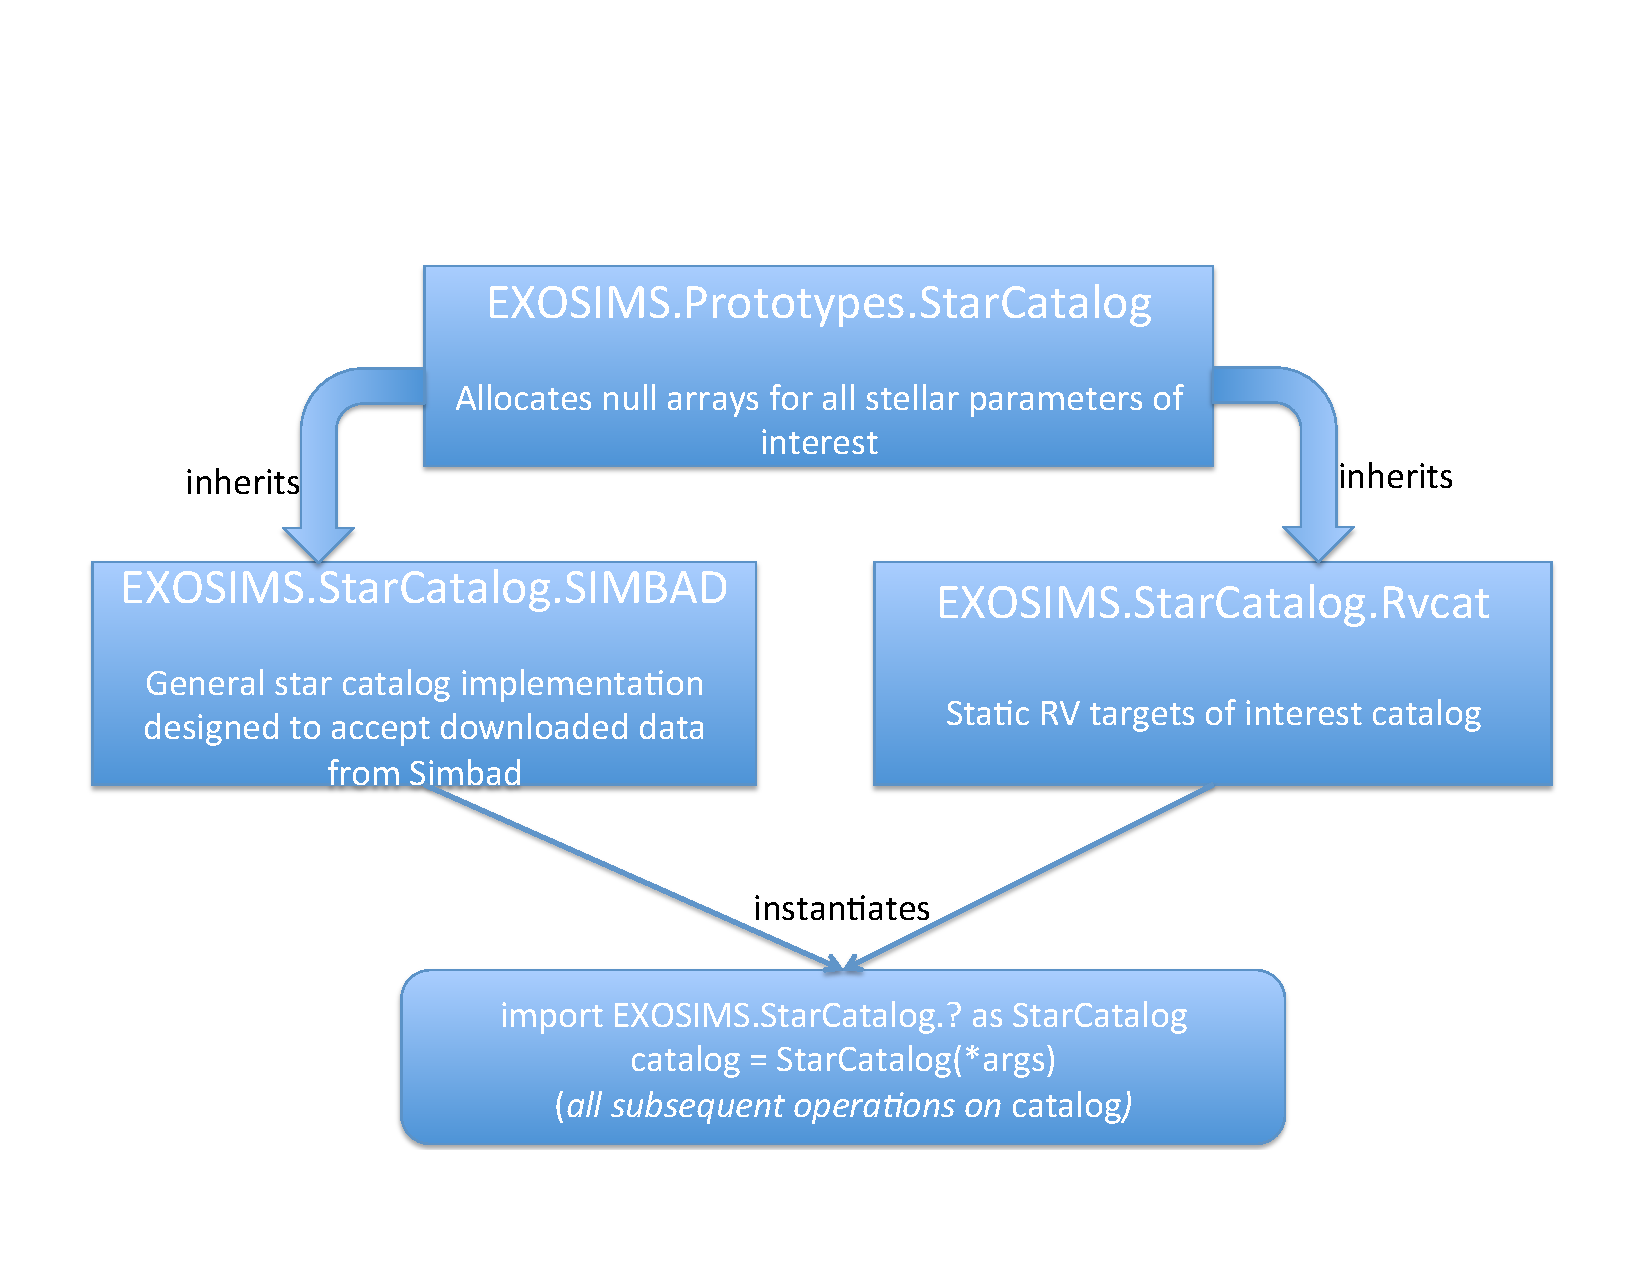
\includegraphics[width=0.75\textwidth]{starcatalog_flowdown}
        \end{tabular}
    \end{center}
    \caption{Schematic of a sample implementation for the three module layers for the Star Catalog module. The Star Catalog prototype (top row) is immutable, specifies the input/output structure of the module along with all common functionality, and is inherited by all Star Catalog class implementations (middle row).  In this case, two different catalog classes are shown: one that reads in data from a SIMBAD catalog dump, and one which contains only information about a subset of known radial velocity targets.  The object used in the simulation (bottom row) is an instance of one of these classes, and can be used in exactly the same way in the rest of the code due to the common input/output scheme.}
    \label{fig:starcatalog_flowdown}
\end{figure}

\begin{figure}[ht]
    \begin{center}
        \begin{tabular}{c}
             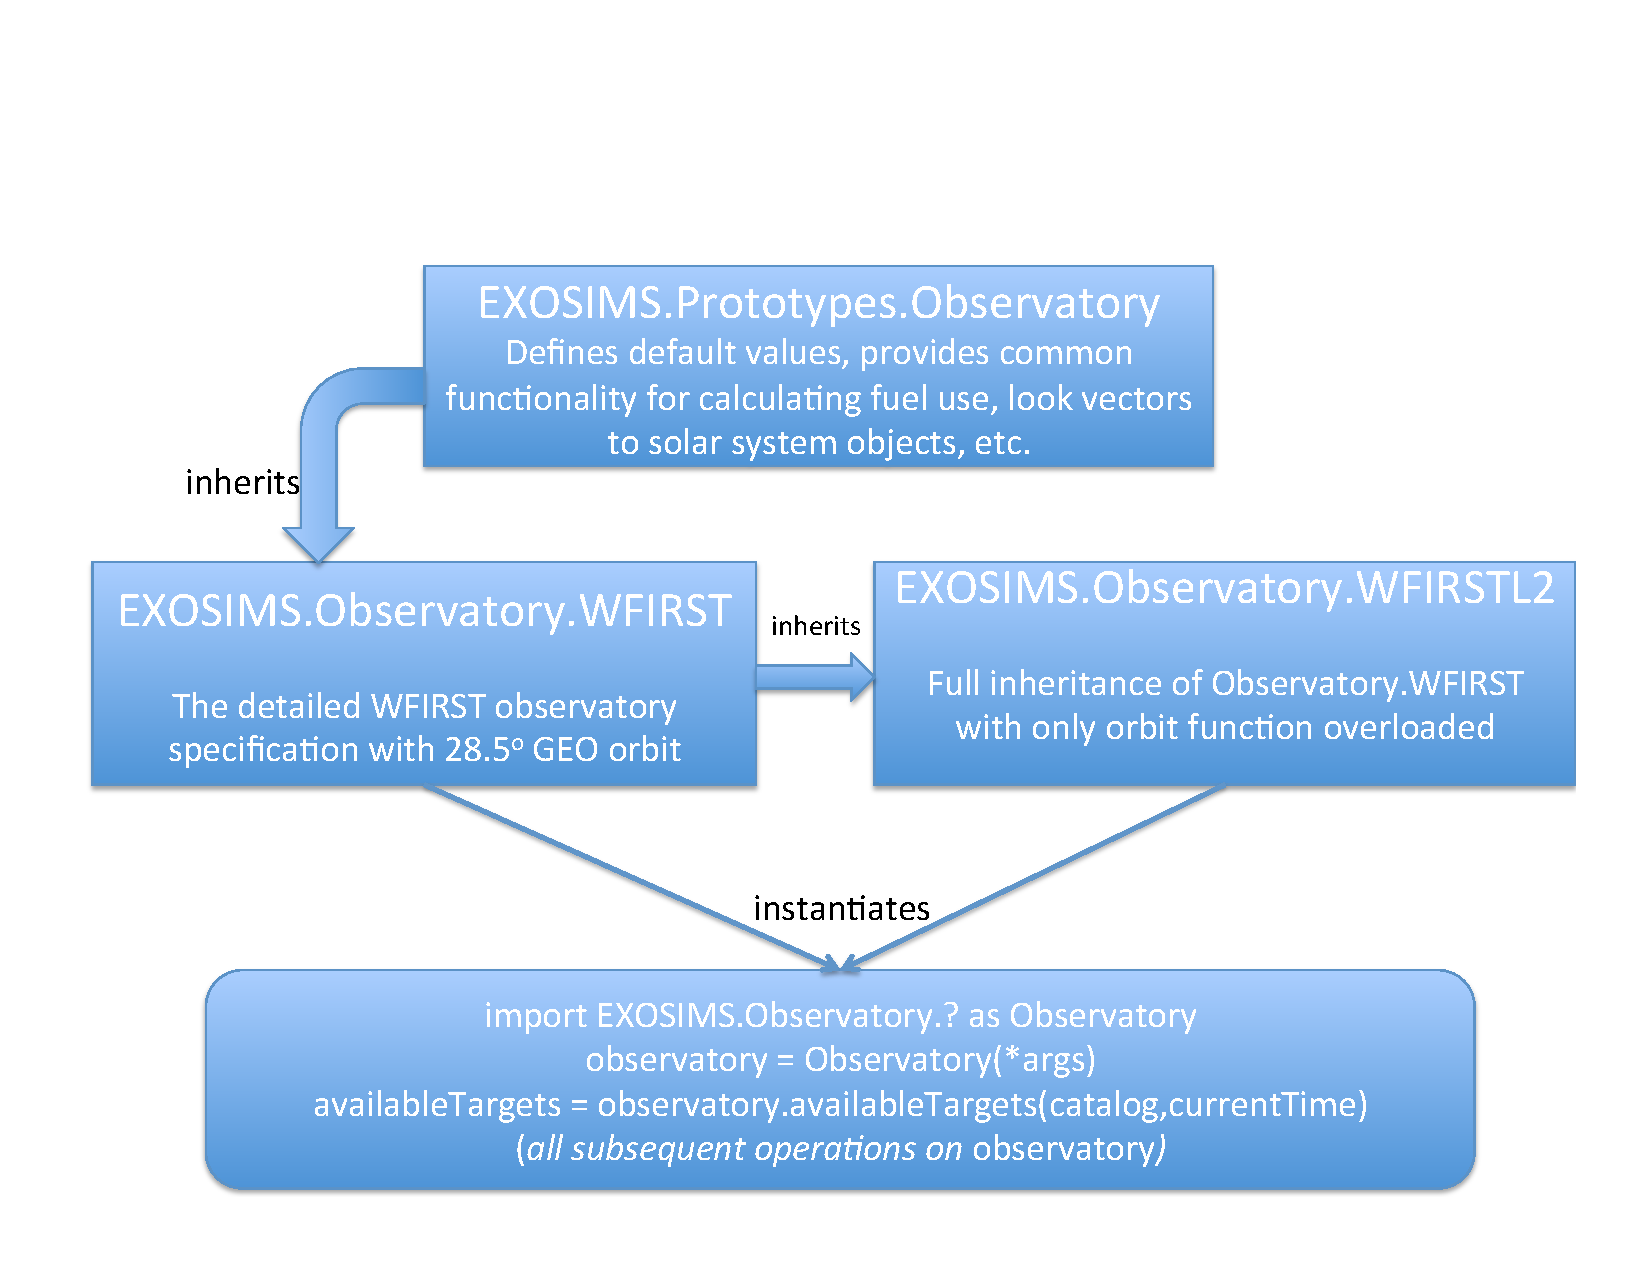
\includegraphics[width=0.75\textwidth]{observatory_flowdown}
        \end{tabular}
    \end{center}
    \caption{Schematic of a sample implementation for the three module layers for the Observatory module. The Observatory prototype (top row) is immutable, specifies the input/output structure of the module along with all common functionality, and is inherited by all Observatory class implementations (middle row).  In this case, two different observatory classes are shown that differ only in the definition of the observatory orbit.  Therefore, the second implementation inherits the first (rather than directly inheriting the prototype) and overloads only the orbit method. The object used in the simulation (bottom row) is an instance of one of these classes, and can be used in exactly the same way in the rest of the code due to the common input/output scheme.}
    \label{fig:observatory_flowdown}
\end{figure}

Figures \ref{fig:starcatalog_flowdown} and \ref{fig:observatory_flowdown} show schematic representations of the three different aspects of a module, using the Star Catalog and Observatory modules as examples, respectively.  Every module has a specific prototype that sets the input/output structure of the module and encodes any common functionality for all module class implementations.  The various implementations inherit the prototype and add/overload any attributes and methods required for their particular tasks, limited only by the preset input/output scheme.  Finally, in the course of running a simulation, an object is generated for each module class selected for that simulation.  The generated objects can be used in exactly the same way in the downstream code, regardless of what implementation they are instances of, due to the strict interface defined in the class prototypes.

For lower level (downstream) modules, the input specification is much more loosely defined than the output specification, as different implementations may draw data from a wide variety of sources.  For example, the star catalog may be implemented as reading values from a static file on disk, or may represent an active connection to a local or remote database.  The output specification for these modules, however, as well as both the input and output for the upstream modules, is entirely fixed so as to allow for generic use of all module objects in the simulation.


\section{Global Specifications}
Common references (units, frames of reference, etc.) are required to ensure interoperability between the modules of EXOSIM.  All of the references listed below must be followed.

\begin{description}
    \item[Common Epoch] \hfill \\ J2000
    \item[Common Reference Frame] \hfill \\ Heliocentric Equatorial (HE)
\end{description}

\subsection{Python Packages} 
EXOSIMS is an open source platform.  As such, packages and modules may be imported and used for calculations within any of the stand-alone modules.  The following commonly used Python packages are used for the WFIRST-specific implementation of EXOSIMS:

\texttt{
\begin{itemize}
    \item astropy
        \begin{itemize}
            \item astropy.constants
            \item astropy.coordinates
            \item astropy.time
            \item astropy.units
        \end{itemize}
    \item copy
    \item importlib
    \item numpy
        \begin{itemize}
            \item numpy.linalg 
        \end{itemize}
    \item os
        \begin{itemize}
            \item os.path 
        \end{itemize}
    \item pickle/cPickle
    \item scipy
        \begin{itemize}
            \item scipy.io
            \item scipy.special
            \item scipy.interpolate
        \end{itemize}
    \item jplephem (\emph{optional})
\end{itemize}
}

Additionally, while not required for running the survey simulation, \verb+matplotlib+ is used for visualization of the results.

\subsection{Coding Conventions}
In order to allow for flexibility in using alternate or user-generated module implementations, the only requirement on any module is that it inherits (either directly or by inheriting another module implementation that inherits the prototype) the appropriate prototype.  It is similarly expected (although not required) that the prototype constructor will be called from the constructor of the newly implemented class.  An example of an Optical System module implementation follows:

\begin{verbatim}
from EXOSIMS.Prototypes.OpticalSystem import OpticalSystem

class ExampleOpticalSystem(OpticalSystem):
    
    def __init__(self, **specs):
                
        OpticalSystem.__init__(self, **specs)
        
        ...

\end{verbatim}

\emph{Note that the filename must match the class name for all modules.}

\subsubsection{Module Type}
It is always possible to check whether a module is an instance of a given prototype, for example:
\begin{verbatim}
isinstance(obj,EXOSIMS.Prototypes.Observatory.Observatory)
\end{verbatim}
However, it can be tedious to look up all of a given object's base classes so, for convenience, every prototype will provide a private variable \verb+_modtype+, which will always return the name of the prototype and should not be overwritten by any module code.  Thus, if the above example evaluates as \verb+True+, \verb+obj._modtype+ will return \verb+Observatory+.

\subsubsection{Callable Attributes}
Certain module attributes must be represented in a way that allows them to be parametrized by other values.  For example, the instrument throughput and contrast are functions of both the wavelength and the angular separation, and so must be encodable as such in the optical system module.  To accommodate this, as well as simpler descriptions where these parameters may be treated as static values, these and other attributes are defined as `callable'.  This means that they must be set as objects that can be called in the normal Python fashion, i.e., \verb+object(arg1,arg2,...)+.  

These objects can be function definitions defined in the code, or imported from other modules.  They can be \href{https://docs.python.org/2/reference/expressions.html#lambda}{lambda expressions} defined inline in the code.  Or they can be callable object instances, such as the various \href{http://docs.scipy.org/doc/scipy/reference/interpolate.html}{scipy interpolants}.  In cases where the description is just a single value, these attributes can be defined as dummy functions that always return the same value, for example:
\begin{verbatim}
def throughput(wavelength,angle):
     return 0.5
\end{verbatim}
or even more simply:
\begin{verbatim}
throughput = lambda wavelength,angle: 0.5
\end{verbatim}
%%%%%%%%%%%%%%%%%%%%%%%%%%%%%%%%%%%%%%%%%%%%%%%%%%%%%%%%%%%%%%%%%%%%
% BACKBONE
%%%%%%%%%%%%%%%%%%%%%%%%%%%%%%%%%%%%%%%%%%%%%%%%%%%%%%%%%%%%%%%%%%%%

\section{Backbone}
By default, the simulation execution will be performed via the backbone.  This will consist of a limited set of functions that will primarily be tasked with parsing the input specification described below, and then creating the specified instances of each of the framework modules, detailed in \S\ref{sec:modules}.  The backbone functionality will primarily be implemented in the MissionSimulation class, whose constructor will take the input script file (\S\ref{sec:inputspec}) and generate instances of all module objects, including the SurveySimulation (\S\ref{sec:surveysim}) and SurveyEnsemble modules, which will contain the functions to run the survey simulations. Any mission-specific execution variations will be introduced by method overloading in the inherited survey simulation implementation. \reffig{fig:instantiation_tree} provides a graphical description of the instantiation order of all module objects.


A simulation specification is a single JSON-formatted (\url{http://json.org/}) file that encodes user-settable parameters and module names.  The backbone will contain a reference specification with \emph{all} parameters and modules set via defaults in the constructors of each of the modules.  In the initial parsing of the user-supplied specification, it will be merged with the reference specification such that any fields not set by the user will be assigned to their reference (default) values.   Each instantiated module object will contain a dictionary called \verb+_outspec+, which, taken together, will form the full specification for the current run (as defined by the loaded modules).  This specification will be written out to a json file associated with the output of every run.  \emph{Any specification added by a user implementation of any module must also be added to the \_outspec dictionary}.  The assembly of the full output specification is provided by MissionSimulation method \verb+genOutSpec+.

The backbone will also contain a specification parser that will check specification files for internal consistency.  For example, if modules carry mutual dependencies, the specification parser will return an error if these are not met for a given specification.  Similarly, if modules are selected with optional top level inputs, warnings will be generated if these are not set in the same specification files.

In addition to the specification parser, the backbone will contain a method for comparing two specification files and returning the difference between them.  Assuming that the files specify all user-settable values, this will be equivalent to simply performing a \verb+diff+ operation on any POSIX system.  The backbone diff function will add in the capability to automatically fill in unset values with their defaults.  For every simulation (or ensemble), an output specification will be written to disk along with the simulation results with all defaults used filled in.

%The backbone will also contain an interactive function to help users generate specification files via a series of questions. 

\subsection{Specification Format}\label{sec:inputspec}
The JSON specification file will contain a series of objects with members enumerating various user-settable parameters, top-level members for universal settings (such as the mission lifetime) and arrays of objects for multiple related specifications, such as starlight suppression systems and science instruments.  The specification file must contain a \verb+modules+ dictionary listing the module names (or paths on disk to user-implemented classes) for all modules.

\begin{verbatim}
{
  "universalParam1": value,
  "universalParam2": value,
  ...
  "starlightSuppressionSystems": [
    {
      "starlightSuppressionSystemNumber": 1,
      "type": "external",
      "detectionTimeMultiplier": value,
      "characterizationTimeMultiplier": value,
      "occulterDiameter": value,
      "NocculterDistances": 2,
      "occulterDistances: [
        {
         "occulterDistanceNumber": 1,
         "occulterDistance": value,
         "occulterBlueEdge": value,
         "occulterRedEdge": value,
         "IWA": value,
         "OWA": value,
         "PSF": "/data/mdo1_psf.fits",
         "throughput": "/data/mdo1_thru.fits",
         "contrast":  "/data1/mdo1_contrast.fits"
        },
        {
         "occulterDistanceNumber": 2,
         "occulterDistance": value,
         "occulterBlueEdge": value,
         "occulterRedEdge": value,
         "IWA": value,
         "OWA": value,
         "PSF": "/data/mdo1_psf.fits",
         "throughput": "/data/mdo1_thru.fits",
         "contrast":  "/data1/mdo1_contrast.fits"
        }
      ],
      "occulterWetMass": value,
      "occulterDryMass": value,
    },
    {
      "starlightSuppressionSystemNumber": 2,
      "type": "internal",
      "IWA": value,
      "OWA": value,
      "PSF": "/data/coron1_psf.fits",
      "throughput": "/data/coron1_thru.fits",
      "contrast":  "/data1/coron1_contrast.fits",
      "detectionTimeMultiplier": value,
      "characterizationTimeMultiplier": value,
      "opticaloh": value
    }
  ],
  "scienceInstruments": [
    {
      "scienceInstrumentNumber": 1,
      "type": "imager-EMCCD",
      "QE": 0.88,
      "darkCurrent": 9e-5,
      "CIC": 0.0013,
      "readNoise": 16,
      "texp": 1000,
      "pixelPitch": 13e-6,
      "focalLength": 240,
      "ENF": 1.414,
      "G_EM": 500
    }
    {
      "scienceInstrumentNumber": 2,
      "type": "IFS-CCD",
      "QE": 0.88,
      "darkCurrent": 9e-5,
      "CIC": 0.0013,
      "readNoise": 3,
      "texp": 1000,
      "Rspec": 70.0,
    }
  ],
  modules: {
    "PlanetPopulation": "HZEarthTwins",
    "StarCatalog": "exocat3",
    "OpticalSystem": "hybridOpticalSystem1",
    "ZodiacalLight": "10xSolZodi",
    "BackgroundSources": "besanconModel",
    "PlanetPhysicalModel": "fortneyPlanets",
    "Observatory": "WFIRSTGeo",
    "TimeKeeping": "UTCtime",
    "PostProcessing": "KLIPpost",
    "Completeness": "BrownCompleteness",
    "TargetList": "WFIRSTtargets",
    "SimulatedUniverse": "simUniverse1",
    "SurveySimulation": "backbone1",
    "SurveyEnsemble": "localIpythonEnsemble"
  }
}
\end{verbatim}

\subsection{Modules Specification}
The final array in the input specification  (\verb+modules+) is a list of all the modules that define a particular simulation.  This is the only part of the specification that will not be filled in by default if a value is missing - each module must be explicitly specified. The order of the modules in the list is arbitrary, so long as they are all present. 

If the module implementations are in the appropriate subfolder in the EXOSIMS tree, then they can be specified by the module name.  However, if you wish to use an implemented module outside of the EXOSIMS directory, then you need to specify it via its full path in the input specification.

\emph{All modules, regardless of where they are stored on disk must inherit the appropriate prototype.}

\subsection{Universal Parameters}
These parameters apply to all simulations, and are described in detail in their specific module definitions:

\begin{itemize}[leftmargin=1in,font={\ttfamily}]
\item[missionLife] (float) The total mission lifetime in $ years $.  When the mission time is equal or greater to this value, the mission simulation stops.
\item[missionPortion] (float) The portion of the mission dedicated to exoplanet science, given as a value between 0 and 1. The mission simulation stops when the total integration time plus observation overhead time is equal to the missionLife $\times$ missionPortion.
\item[keepStarCatalog] (boolean) Boolean representing whether to delete the star catalog after assembling the target list.  If true, object reference will be available from TargetList object.
\item[minComp] (float) Minimum completeness value for inclusion in target list. 
\item[lam] (float) Detection central wavelength in $ nm $.
\item[deltaLam] (float) Detection bandwidth in $ nm $.
\item[BW] (float) Detection bandwidth fraction = $\Delta\lambda/\lambda$.
\item[specLam] (float) Spectrograph central wavelength in $ nm $.
\item[specDeltaLam] (float) Spectrograph bandwidth in $ nm $.
\item[specBW] (float) Spectrograph bandwidth fraction = $\Delta\lambda_s/\lambda_s$.
\item[obscurFac] (float) Obscuration factor due to secondary mirror and spiders.
\item[shapeFac] (float)  Telescope aperture shape factor.
\item[pupilDiam] (float) Entrance pupil diameter in $m$.
\item[pupilArea] (float) Entrance pupil area in $m^2$.
\item[IWA] (float) Fundamental Inner Working Angle in $ arcsec $. No planets can ever be observed at smaller separations.
\item[OWA] (float) Fundamental Outer Working Angle in $ arcsec $. Set to $ Inf $ for no OWA. JSON values of 0 will be interpreted as $ Inf $.
\item[dMagLim] (float) Fundamental limiting $\Delta$mag (difference in magnitude between star and planet). 
\item[telescopeKeepout] (float) Telescope keepout angle in $ deg $
\item[attenuation] (float) Non-coronagraph attenuation, equal to the throughput of the optical system without the coronagraph elements.
\item[intCutoff] (float)  Maximum allowed integration time in $ day $. No integrations will be started that would take longer than this value.
\item[FAP] (float) Detection false alarm probability
\item[MDP] (float) Missed detection probability
\item[SNimag] (float) Signal to Noise Ratio for imaging/detection.
\item[SNchar] (float) Signal to Noise Ratio for characterization.
\item[arange] (float) 1$\times$2 list of semi-major axis range in $ AU $. 
\item[erange] (float) 1$\times$2 list of eccentricity range.
\item[Irange] (float) 1$\times$2 list of inclination range in $ deg $.  
\item[Orange] (float) 1$\times$2 list of ascension of the ascending node range in $ deg $.  
\item[wrange] (float) 1$\times$2 list of argument of perigee range in $ deg $. 
\item[prange] (float) 1$\times$2 list of planetary geometric albedo range.  
\item[Rprange] (float) 1$\times$2 list of planetary radius range in Earth radii.  
\item[Mprange] (float) 1$\times$2 list of planetary mass range in Earth masses.  
\item [scaleOrbits] (boolean) True means planetary orbits are scaled by the square root of stellar luminosity. 
\item[constrainOrbits] (boolean) True means planetary orbits are constrained to never leave the semi-major axis range (arange).
\item[missionStart] (float) Mission start time in $ MJD $. 
\item[extendedLife] (float) Extended mission time in $ years $.  Extended life typically differs from the primary mission in some way---most typically only revisits are allowed
\item[settlingTime] (float) Amount of time needed for observatory to settle after a repointing in $ day $.           
\item[thrust] (float) Occulter slew thrust in $ mN $.
\item[slewIsp] (float) Occulter slew specific impulse in $ s $.
\item[scMass] (float) Occulter (maneuvering spacecraft) initial wet mass in $ kg $. 
\item[dryMass] (float) Occulter (maneuvering spacecraft) dry mass in $ kg $. 
\item[coMass] (float) Telescope (or non-maneuvering spacecraft) mass in $ kg $. 
\item[skIsp] (float) Specific impulse for station keeping in $ s $. 
\item[defburnPortion] (float) Default burn portion for slewing.
\item[spkpath] (string) Full path to SPK kernel file.
\item[forceStaticEphem]  (boolean) Force use of static solar system ephemeris if set to True, even if jplephem module is present.
\end{itemize}


\section{Module Specifications}\label{sec:modules}
The lower level modules include Planet Population, Star Catalog, Optical System, Zodiacal Light, Background Sources, Planet Physical Model, Observatory, Time Keeping, and Post-Processing.  These modules encode and/or generate all of the information necessary to perform mission simulations.  The specific mission design determines the functionality of each module, while inputs and outputs of these modules remain the same (in terms of data type and variable representations).  

The upstream modules include Completeness, Target List, Simulated Universe, Survey Simulation and Survey Ensemble. These modules perform methods which require inputs from one or more downstream modules as well as calling function implementations in other upstream modules. 

This section defines the functionality, major tasks, input, output, and interface of each of these modules. Every module constructor must always accept a keyword dictionary (\verb+**spec+) representing the contents of the specification JSON file organized into a Python dictionary. The descriptions below list out specific keywords that are pulled out by the prototype constructors of each of the modules, but implemented constructors may include additional keywords (so long as they correctly call the prototype constructor).  In all cases, if a given \verb+key:value+ pair is missing from the dictionary, the appropriate object attributes will be assigned the default values listed.


% PLANET POPULATION

\subsection{Planet Population}
The Planet Population module encodes the density functions of all required planetary parameters, both physical and orbital. These include semi-major axis, eccentricity, orbital orientation, radius, mass, and geometric albedo (see \S\ref{sec:pdfs}). Certain parameter models may be empirically derived while others may come from analyses of observational surveys.  This module also encodes the limits on all parameters to be used for sampling the distributions and determining derived cutoff values such as the maximum target distance for a given instrument's IWA.

\begin{figure}[ht]
    \begin{center}
        \begin{tabular}{c}
             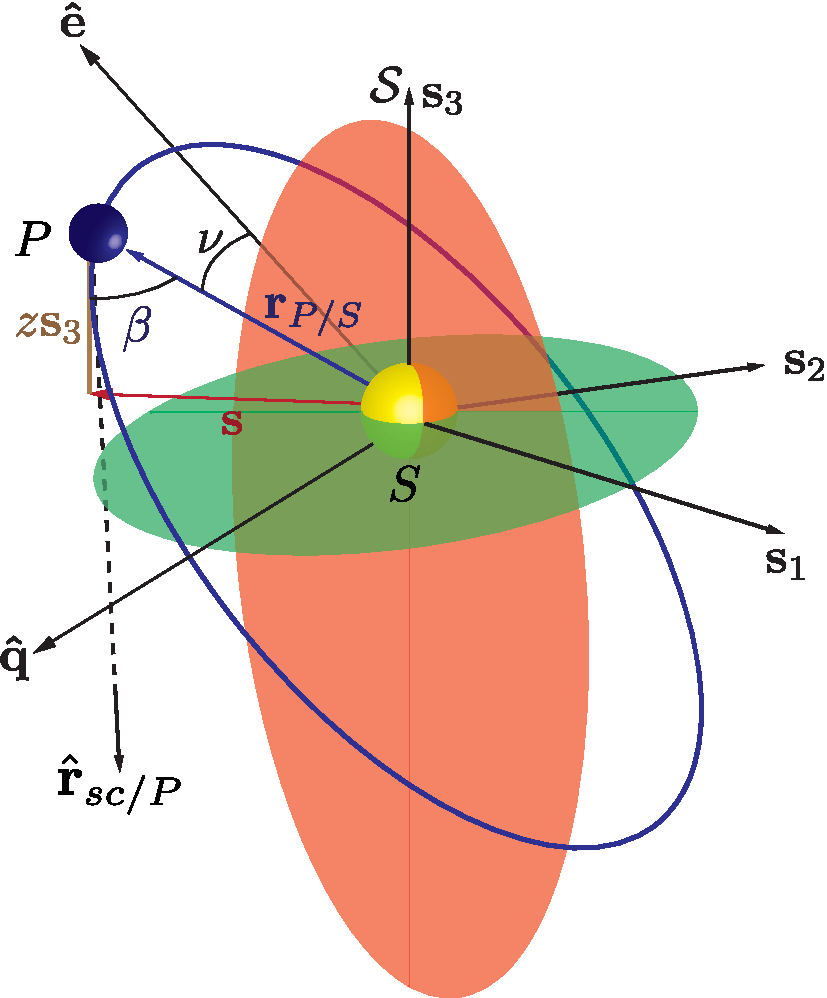
\includegraphics[width=0.6\textwidth]{orbit_diagram}
        \end{tabular}
    \end{center}
    \caption{\label{fig:orbit_diagram} Definition of reference frames and coordinates of simulated exosystems.  The observer lies along the negative $\mf s_3$ axis so that the observer-star unit vector is $+\mf s_3$.}
\end{figure}

The coordinate system of the simulated exosystems is defined as in \reffig{fig:orbit_diagram}.  The observer looks at the target star along the $\mathbf{s}_3$ axis, located at a distance $-d\mathbf{s}$ from the target at the time of observation. The argument of periapse, inclination,  and longitude of the ascending node ($\omega, I, \Omega$) are defined as a 3-1-3 rotation about the unit vectors defining the $\mathcal{S}$ reference frame.  This rotation defines the standard Equinoctial reference frame ($\mfhat{e}, \mfhat{q}, \mfhat{h}$), with the true anomaly ($\nu$) measured from $\mfhat{e}$).  The planet-star orbital radius vector $\mf r_{P/S}$ is projected into the $\mf s_1, \mf s_2$ plane as the projected separation vector $\mf s$, with magnitude $s$, and the phase (star-planet-observer) angle ($\beta$) is closely approximated by the angle between $\mf r_{P/s}$ and its projection onto $\mf s_3$.

The Planet Population module does not model the physics of planetary orbits or the amount of light reflected or emitted by a given planet, but rather encodes the statistics of planetary occurrence and properties. 

\label{sec:planetpopulation}
\subsubsection{Planet Population Object Attribute Initialization} 
\subsubsection*{Inputs}
The following are all entries in the passed specs dictionary (derived from the JSON script file or another dictionary).  Values not specified will be replaced with defaults, as listed.  It is important to note that many of these (in particular mass and radius) may be mutually dependent, and so some implementation may choose to only use some for inputs and set the rest via the physical models.

\begin{itemize}
\item
\begin{description}
    \item[arange] \hfill \\
    1$\times$2 list of semi-major axis range in $ AU $. Default value is [0.01, 100]
    \item[erange] \hfill \\
    1$\times$2 list of eccentricity range.  Default value is [0.01,0.99]
    \item[Irange] \hfill \\
    1$\times$2 list of inclination range in $ deg $.  Default value is [0,180]
    \item[Orange] \hfill \\
    1$\times$2 list of ascension of the ascending node range in $ deg $.  Default value is [0,360]
    \item[wrange] \hfill \\
    1$\times$2 list of perigee range in $ deg $.  Default value is [0,360]
    \item[prange] \hfill \\
    1$\times$2 list of planetary geometric albedo range.  Default value is [0.1,0.6]
    \item[Rprange] \hfill \\
    1$\times$2 list of planetary Radius in Earth radii.  Default value is [1, 30]
    \item[Mprange] \hfill \\
    1$\times$2 list of planetary mass in Earth masses.  Default value is [1, 4131]
    \item [scaleOrbits] \hfill \\
    Boolean where True means planetary orbits are scaled by the square root of stellar luminosity. Default value is False.
    \item[constrainOrbits] \hfill \\
    Boolean where True means planetary orbits are constrained to never leave the semi-major axis range (arange). Default value is False.
\end{description}
\end{itemize}

\subsubsection*{Attributes}
\begin{itemize}
    \item
    \begin{description}
        \item[arange (astropy Quantity 1$\times$2 array):] \hfill \\
        Semi-major axis range defined as [a\_min, a\_max] in units of $ AU $
        \item[erange (1$\times$2 ndarray):] \hfill \\
        Eccentricity range defined as [e\_min, e\_max]
        \item[Irange (astropy Quantity 1$\times$2 array):] \hfill \\
        Planetary orbital inclination range defined as [I\_min, I\_max] in units of $ deg $
        \item[Orange (astropy Quantity 1$\times$2 array):] \hfill \\
        Right ascension of the ascending node range defined as [O\_min, O\_max] in units of $ deg $
        \item[wrange (astropy Quantity 1$\times$2 array):] \hfill \\
        Argument of perigee range defined as [w\_min, w\_max] in units of $ deg $
        \item[prange (1$\times$2 ndarray):] \hfill \\
        Planetary geometric albedo range defined as [p\_min, p\_max]
        \item[Rprange (astropy Quantity 1$\times$2 array):] \hfill \\
        Planetary radius range defined as [R\_min, R\_max] in units of $ km $
        \item[Mprange (astropy Quantity 1$\times$2 array):] \hfill \\
        Planetary mass range defined as [Mp\_min, Mp\_max] in units of $ kg $
        \item[rrange (astropy Quantity 1$\times$2 array):] \hfill \\
        Planetary orbital radius range defined as [r\_min, r\_max] derived from PlanetPopulation.arange and PlanetPopulation.erange, in units of $ AU $
        \item [scaleOrbits (boolean):] \hfill \\
        Boolean where True means planetary orbits are scaled by the square root of stellar luminosity.
        \item[constrainOribts (boolean):] \hfill \\
        Boolean where True means planetary orbits are constrained to never leave the semi-major axis range (arange). If set to True, an additional method (\verb+gen_eccen_from_sma+) must be provided by the implementation---see below.
        \item[PlanetPhysicalModel (object):] \hfill \\     
            PlanetPhysicalModel class object
    \end{description}
\end{itemize}

\subsubsection{Planet Population Value Generators} \label{sec:pdfs}
For each of the parameters represented by the input attributes, the planet population object will provide a method that returns random values for the attribute, within the ranges specified by the attribute (so that, for example, there will be a \verb+gen_sma+ method corresponding to \verb+arange+, etc.).  Each of these methods will take a single input of the number of values to generate.  These methods will encode the probability density functions representing each parameter, and use either a rejection sampler or other (numpy or scipy) provided sampling method to generate random values.  All returned values will have the same type/default units as the attributes. 

In cases where values need to be sampled jointly (for example if you have a joint distribution of semi-major axis and planetary radius) then the sampling will be done by a helper function which stores the last sampled values in memory, and the individual functions (i.e., \verb+gen_sma+ and \verb+gen_radius+) will act as getters for the values.  In cases where there is a deterministic calculation of one parameter from another (as in mass calculated from radius) this will be provided separately in the Planet Physical module. Any non-standard distribution functions being sampled by one of these methods should be created as object attributes in the implementation constructor so that they are available to other modules.
\\\\
The methods are:

\begin{itemize}
    \item 
    \begin{description}
        \item[gen\_sma] \hfill \\
        Returns semi-major axis values (astropy Quantity initially set in $ AU $)
        \item[gen\_eccen] \hfill \\
        Returns eccentricity values (numpy ndarray)
        \item[gen\_w] \hfill \\
        Returns argument of perigee values (astropy Quantity initially set in $ deg $)
        \item[gen\_O] \hfill \\
        Returns longitude of the ascending node values (astropy Quantity initially set in $ deg $)
        \item[gen\_radius] \hfill \\
        Returns planetary radius values  (astropy Quantity initially set in $ m $)
        \item[gen\_mass] \hfill \\
        Returns planetary mass values (astropy Quantity initially set in $ kg $)
        \item[gen\_albedo] \hfill \\
        Returns planetary geometric albedo (numpy ndarray)
        \item[gen\_I] \hfill \\
        Returns values of orbital inclination (astropy Quantity initially set in $ deg $)
        \item[gen\_eccen\_from\_sma] \hfill \\
        Required only for populations that can take a \verb+constrainOrbits=True+ input. Takes an additional argument of array of semi-major axis values (astropy Quantity). Returns eccentricity values (numpy ndarray) such that $a(1-e) \ge  a_\textrm{min}$ and $a(1+e) \le a_\textrm{max}$.
    \end{description}
\end{itemize}

% PLANET PHYSICAL MODEL 

\subsection{Planet Physical Model} \label{sec:planetphysicalmodel}
The Planet Physical Model module contains models of the light emitted or reflected by planets in the wavelength bands under investigation by the current mission simulation.  It takes as inputs the physical quantities sampled from the distributions in the Planet Population module and generates synthetic spectra (or band photometry, as appropriate).  The specific implementation of this module can vary greatly, and can be based on any of the many available planetary geometric albedo, spectra and phase curve models.  As required, this module also provides physical models relating dependent parameters that cannot be sampled independently (for example density models relating plant mass and radius).  While the specific methods will depend highly on the physical models being used, the prototype provides four stubs that will be commonly useful:

\begin{itemize}
    \item 
    \begin{description}
        \item[calc\_albedo\_from\_sma] \hfill \\
        Provides a method to calculate planetary geometric albedo as a function of the semi-major axis
        \item[calc\_mass\_from\_radius] \hfill \\
        Provides a method to calculate planetary masses from their radii
        \item[calc\_radius\_from\_mass] \hfill \\
        Provides a method to calculate planetary radii from their masses
        \item[calc\_Phi] \hfill \\
        Provides a method to calculate the value of the planet phase function given the phase.  The prototype implementation uses the Lambert phase function.
    \end{description}
\end{itemize}



% STAR CATALOG

\subsection{Star Catalog} \label{sec:starcatalog}
The Star Catalog module includes detailed information about potential target stars drawn from general databases such as SIMBAD, mission catalogs such as Hipparcos, or from existing curated lists specifically designed for exoplanet imaging missions.  Information to be stored, or accessed by this module will include target positions and proper motions at the reference epoch, catalog identifiers (for later cross-referencing), bolometric luminosities, stellar masses, and magnitudes in standard observing bands.  Where direct measurements of any value are not available, values are synthesized from ancillary data and empirical relationships, such as color relationships and mass-luminosity relations.

This module does not provide any functionality for picking the specific targets to be observed in any one simulation, nor even for culling targets from the input lists where no observations of a planet could take place.  This is done in the Target List module as it requires interactions with the Planet Population (to determine the population of interest), Optical System (to define the capabilities of the instrument), and Observatory (to determine if the view of the target is unobstructed) modules.

\subsubsection{Star Catalog Object Attribute Initialization} 
The Star Catalog prototype creates empty 1D NumPy ndarrays for each of the output quantities listed below.  Specific Star Catalog modules must populate the values as appropriate.  Note that values that are left unpopulated by the implementation will still get all zero array, which may lead to unexpected behavior.

\subsubsection*{Inputs}
\begin{itemize}
    \item 
    \begin{description}
        \item[star catalog information] \hfill \\
        Information from an external star catalog (left deliberately vague as these can be anything).
    \end{description}
\end{itemize}

\subsubsection*{Attributes}
\begin{itemize}
    \item 
    \begin{description}
        \item[Name (string ndarray)] \hfill \\
        Star names
        \item[Spec (string ndarray)] \hfill \\
        Spectral types
        \item[Umag (float ndarray)] \hfill \\
        U magnitude
        \item[Bmag (float ndarray)] \hfill \\
        B magnitude
        \item[Vmag (float ndarray)] \hfill \\
        V magnitude
        \item[Rmag (float ndarray)] \hfill \\
        R magnitude
        \item[Imag (float ndarray)] \hfill \\
        I magnitude
        \item[Jmag (float ndarray)] \hfill \\
        J magnitude
        \item[Hmag (float ndarray)] \hfill \\
        H magnitude
        \item[Kmag (float ndarray)] \hfill \\
        K magnitude
        \item[BV (float ndarray)] \hfill \\
        B-V Johnson magnitude
        \item[MV (float ndarray)] \hfill \\
        Absolute V magnitude
        \item[BC (float ndarray)] \hfill \\
        Bolometric correction
        \item[L (float ndarray)] \hfill \\
        Stellar luminosity in Solar luminosities
        \item[Binary\_Cut (boolean ndarray)] \hfill \\ Booleans where True is a star with a companion closer than $ 10 arcsec $




        \item[dist (astropy Quantity array)] \hfill \\
        Distance to star in units of $ pc $. Defaults to 1.
        \item[parx (astropy Quantity array)] \hfill \\
        Parallax in units of $ mas $. Defaults to 1000.
        \item[coords (astropy SkyCoord array)] \hfill \\
        \href{http://astropy.readthedocs.org/en/latest/api/astropy.coordinates.SkyCoord.html}{SkyCoord object} containing right ascension, declination, and distance to star in units of $ deg $, $ deg $, and $ pc $.
        \item[pmra (astropy Quantity array)] \hfill \\
        Proper motion in right ascension in units of $ mas/year $
        \item[pmdec (astropy Quantity array)] \hfill \\
        Proper motion in declination in units of $ mas/year $
        \item[rv (astropy Quantity array)] \hfill \\
        Radial velocity in units of $ km/s $
    \end{description}
\end{itemize}

\subsection{Optical System}
The Optical System module contains all of the necessary information to describe the effects of the telescope and starlight suppression system on the target star and planet wavefronts.  This requires encoding the design of both the telescope optics and the specific starlight suppression system, whether it be an internal coronagraph or an external occulter.  The encoding can be achieved by specifying Point Spread Functions (PSF) for on- and off-axis sources, along with angular separation and wavelength dependent contrast and throughput definitions.  At the opposite level of complexity, the encoded portions of this module may be a description of all of the optical elements between the telescope aperture and the imaging detector, along with a method of propagating an input wavefront to the final image plane.  Intermediate implementations can include partial propagations, or collections of static PSFs representing the contributions of various system elements.  The encoding of the optical train will allow for the extraction of specific bulk parameters including the instrument inner working angle (IWA), outer working angle (OWA), and mean and max contrast and throughput.

Finally, the Optical System must also include a description of the science instrument.  The baseline instrument is assumed to be an imaging spectrometer.  The encoding must provide the spatial and wavelength coverage of the instrument as well as sampling for each, along with detector details such as read noise, dark current, and readout cycle.

The Optical System module has four methods used in simulation.  \verb+calc_maxintTime+ is called from the Target List module to calculate the maximum integration time for each star in the target list (see \S\ref{sec:calcmaxintTimetask}).  \verb+calc_intTime+ and \verb+calc_charTime+ are called from the Survey Simulation module to calculate integration and characterization times for a target system (see \S\ref{sec:calcintTimetask} and \S\ref{sec:calccharTimetask}). \verb+Cp_Cb+ is called by \verb+calc_intTime+ and \verb+calc_charTime+ to calculate the electron count rates for planet signal and background noise (see \S\ref{sec:CpCbtask}).
The inputs and outputs for the Optical System methods are depicted in \reffig{fig:opticalsysmodule}.

\begin{figure}[ht]
    \begin{center}
        \begin{tabular}{c}
            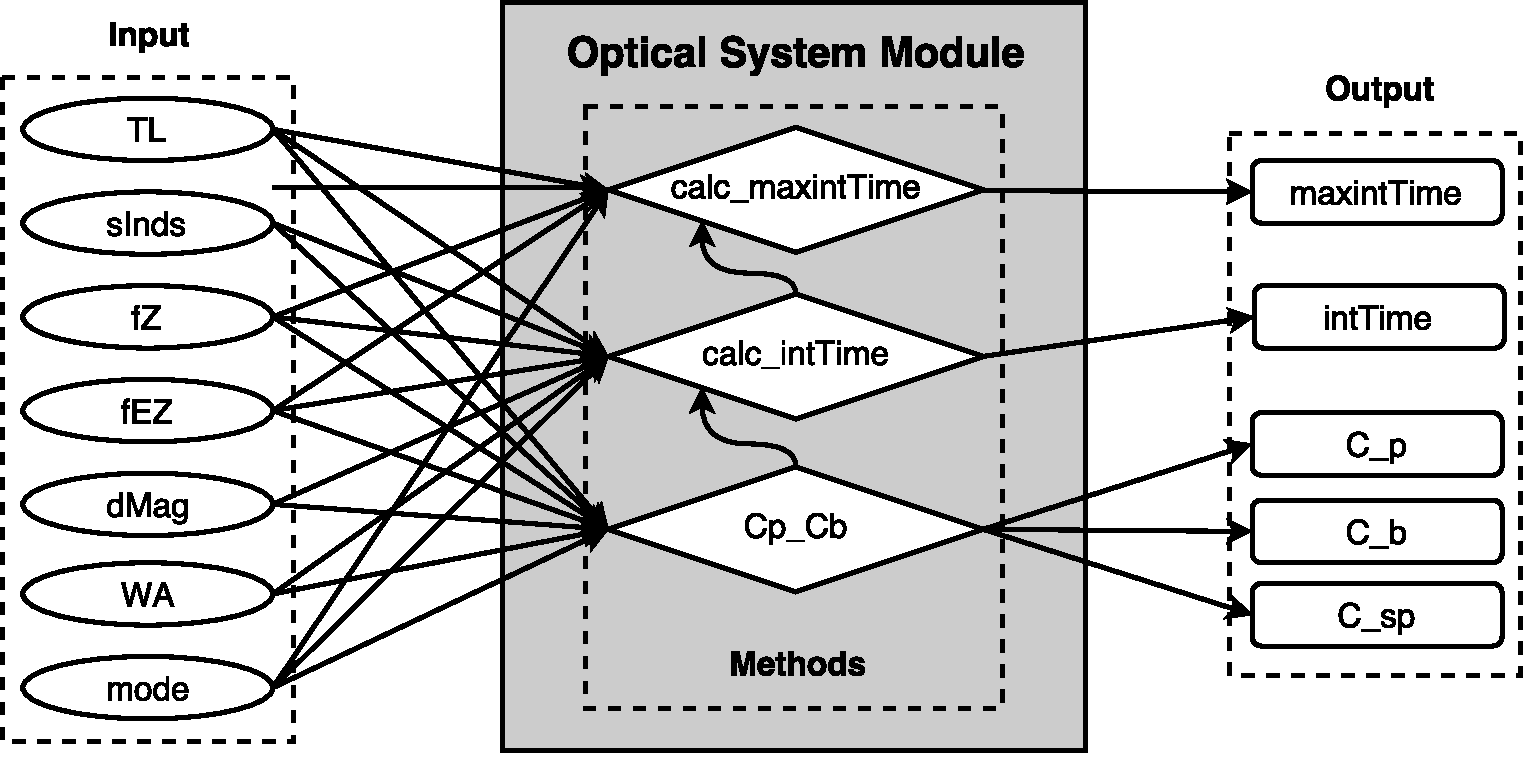
\includegraphics[width=\textwidth]{OpticalSysTasks2}
        \end{tabular}
    \end{center}
    \caption{\label{fig:opticalsysmodule} Depiction of Optical System module methods including inputs and outputs (see \S\ref{sec:calcmaxintTimetask}, S\ref{sec:calcintTimetask}, S\ref{sec:calccharTimetask} and \S\ref{sec:CpCbtask}).}
\end{figure}


\label{sec:opticalsystem}
\subsubsection{Optical System Object Attribute Initialization} 

The specific set of inputs to this module will vary based on the simulation approach used.  Here we define the specification for the case where static PSF(s), derived from external diffraction modeling, are used to describe the system.  Note that some of the inputs are coronagraph or occulter specific, and will be expected based on the "internal" or "external" starlight suppression system keyword, respectively.


\subsubsection*{Inputs}
Information from simulation specification JSON file organized into a Python dictionary.  For multiple systems, there will be an array of dictionaries. If the below \verb+key:value+ pairs are missing from the input specification, the Optical System object attributes will be assigned the default values listed. The following are all entries in the passed specs dictionary.

\begin{itemize}
    \item 
\begin{description}
    \item[obscurFac] \hfill \\
    Obscuration factor due to secondary mirror and spiders. Default value is 0.1.
    \item[shapeFac] \hfill \\
    Shape factor of the unobscured pupil area, so that $ shapeFac \times pupilDiam^2  \times (1-obscurFac) = pupilArea $. Default value is $ \frac{\pi}{4} $.
    \item[pupilDiam] \hfill \\
    Entrance pupil diameter in  $ m $. Default value is 4.
    \item[telescopeKeepout] \hfill \\
    Telescope keepout angle in $ deg $. Default value is 45.
    \item[attenuation] \hfill \\
    Non-coronagraph attenuation, equal to the throughput of the optical system without the coronagraph elements. Default value is 0.57.
    \item[intCutoff] \hfill \\
    Maximum allowed integration time in $ day $. No integrations will be started that would take longer than this value. Default value is 50.
    \item[Npix] \hfill \\
    Number of noise pixels. Default value is 14.3.
    \item[Ndark] \hfill \\
    Number of dark frames used. Default value is 10.
    \item[IWA] \hfill \\
    Fundamental Inner Working Angle in $ arcsec $. No planets can ever be observed at smaller separations. If not set, defaults to smallest IWA of all starlightSuppressionSystems.
    \item[OWA] \hfill \\
    Fundamental Outer Working Angle in $ arcsec $. Set to $ Inf $ for no OWA. If not set, defaults to largest OWA of all starlightSuppressionSystems.  JSON values of 0 will be interpreted as $ Inf $.
    \item[dMagLim] \hfill \\
    Fundamental limiting $ \Delta$mag (difference in magnitude between star and planet). Default value is 20.
    \item[scienceInstruments] \hfill\\ List of dictionaries containing specific attributes of all science instruments. For each instrument, if the below attributes are missing from the dictionary, they will be assigned the default values listed, or any value directly passed as input to the class constructor. In case of multiple instruments, specified wavelength values (lam, deltaLam, BW) of the first instrument become the new default values.
    \begin{description}
    \item[type] \hfill\\ (Required) String indicating type of system.  Standard values are `imaging' and `spectro'.
    \item[lam] \hfill \\
    Central wavelength $\lambda$ in $ nm $. Default value is 500. 
    \item[deltaLam] \hfill \\
    Bandwidth $ \Delta\lambda $ in $ nm $. Defaults to lambda $ \times $ BW (defined hereunder).
    \item[BW] \hfill \\ Bandwidth fraction $(\Delta\lambda/\lambda)$. Only applies when deltaLam is not specified. Default value is 0.2.
    \item[pitch] \hfill \\
    Pixel pitch in $ m $. Default value is 13e-6. 
    \item[focal] \hfill \\
    Focal length in $ m $. Default value is 140. 
    \item[idark] \hfill \\
    Detector dark-current rate in $ electrons /s /pix $. Default value is 9e-5. 
    \item[texp] \hfill \\
    Exposure time in $ s/frame $. Default value is 1e3. 
    \item[sread] \hfill \\
    Detector read noise in $ electrons/frame $. Default value is 3. 
    \item[CIC] \hfill \\
    (Specific to CCDs) Clock-induced-charge in $ electrons/pix/frame $. Default value is 0.0013. 
    \item[ENF] \hfill \\
    (Specific to EM-CCDs) Excess noise factor. Default value is 1. 
    \item[Gem] \hfill \\
    (Specific to EM-CCDs) Electron multiplication gain. Default value is 1. 
    \item[Rs] \hfill \\
    (Specific to spectrometers) Spectral resolving power defined as $\lambda/d\lambda$. Default value is 70. 
    \item[QE] \hfill \\
    Detector quantum efficiency: either a scalar for constant QE, or a two-column array for wavelength-dependent QE, where the first column contains the wavelengths in $ nm $. The ranges on all parameters must be consistent with the values for lam and deltaLam inputs. May be data or FITS filename. Default is scalar 0.9. 
    \end{description}
    \item[starlightSuppressionSystems] \hfill\\ List of dictionaries containing specific attributes of all starlight suppression systems. For each system, if the below attributes are missing from the dictionary, they will be assigned the default values listed, or any value directly passed as input to the class constructor.
    \begin{description}
    \item[type] \hfill\\ (Required) String indicating the system type (e.g. internal, external, hybrid), should also contain the type of science instrument it can be used with (e.g. imaging, spectro).
    \item[throughput] \hfill \\
    System throughput: either a scalar for constant throughput, a two-column array for angular separation-dependent throughput, where the first column contains the separations in $ arcsec $, or a 2D array for angular separation- and wavelength- dependent throughput, where the first column contains the angular separation values in $ arcsec $ and the first row contains the wavelengths in $ nm $.  The ranges on all parameters must be consistent with the values for the IWA, OWA, lam and deltaLam inputs.  May be data or FITS filename. Default is scalar 1e-2.
    \item[contrast] \hfill \\
    System contrast: either a scalar for constant contrast, a two-column array for angular separation-dependent contrast, where the first column contains the separations in $ arcsec $, or a 2D array for angular separation- and wavelength- dependent contrast, where the first column contains the angular separation values in as and the first row contains the wavelengths in $ nm $.  The ranges on all parameters must be consistent with the values for the IWA, OWA, lam and deltaLam inputs. May be data or FITS filename. Default is scalar 1e-9.
    \item[IWA] \hfill \\
     Inner Working Angle of this system in $ arcsec $. If not set, or if too small for this system contrast/throughput definitions, defaults to smallest WA of contrast/throughput definitions.
    \item[OWA] \hfill \\
    Specific Outer Working Angle of this system in $ arcsec $. Set to $ Inf $ for no OWA. If not set, or if too large for this system contrast/throughput definitions, defaults to largest WA of contrast/throughput definitions.  JSON values of $ 0 $ will be interpreted as $ Inf $.
    \item[PSF] \hfill \\
    Instrument point spread function. Either a 2D array of a single-PSF, or a 3D array of wavelength-dependent PSFs. May be data or FITS filename. Default is numpy.ones((3,3)).
    \item[samp] \hfill \\
    Sampling of the PSF in $ arcsec $ per pixel. Default value is 10.
    \item[ohTime] \hfill \\
    Optical system overhead time in $ day $.  Default value is $ 1 $ day.  This is the (assumed constant) amount of time required to set up the optical system (i.e., dig the dark hole or do fine alignment with the occulter).  It is added to every observation, and is separate from the observatory overhead defined in the observatory module, which represents the observatory's settling time.  Both overheads are added to the integration time to determine the full duration of each detection observation.
    \item[imagTimeMult]\hfill \\
    Duty cycle of a detection observation.  If only a single integration is required for the initial detection observation, then this value is 1.  Otherwise, it is equal to the number of discrete integrations needed to cover the full field of view (i.e., if a shaped pupil with a dark hole that covers 1/3 of the field of view is used for detection, this value would equal 3).  Defaults to 1.
    \item[charTimeMult]\hfill \\
    Characterization duty cycle.  If only a single integration is required for the initial detection observation, then this value is 1.  Otherwise, it is equal to the number of discrete integrations needed to cover the full wavelength band and all required polarization states.  For example, if the band is split into three sub-bands, and there are two polarization states that must be measured, and each of these must be done sequentially, then this value would equal 6.  However, if the three sub-bands could be observed at the same time (e.g., by separate detectors) then the value would by two (for the two polarization states). Defaults to 1.
    \item[occulterDiameter]\hfill \\
    Occulter diameter in $ m $.  Measured petal tip-to-tip.
    \item [NocculterDistances]\hfill \\
    Number of telescope separations the occulter operates over (number of occulter bands). If greater than 1, then the occulter description is an array of dicts.
    \item[occulterDistance]\hfill \\
    Telescope-occulter separation in $km$.
    \item[occulterBlueEdge]\hfill \\
    Occulter blue end of wavelength band in $nm$.
    \item[occulterRedEdge]\hfill \\
    Occulter red end of wavelength band in $nm$.
    \end{description}
\end{description}
\end{itemize}
For all values that may be either scalars or interpolants, in the case where scalar values are given, the optical system module will automatically wrap them in lambda functions so that they become callable (just like the interpolant) but will always return the same value for all arguments.  The inputs for interpolants may be filenames (full absolute paths) with tabulated data, or NumPy ndarrays of argument and data (in that order in rows so that input[0] is the argument and input[1] is the data).  When the input is derived from a JSON file, these must either be scalars or filenames.

The starlight suppression system and science instrument dictionaries can contain any other attributes required by a particular optical system implementation.  The only significance of the ones enumerated above is that they are explicitly checked for by the prototype constructor, and cast to their expected values.

%In cases where there is only one starlight suppression system and/or one science instrument, all values from those dictionaries are copied directly to the OpticalSystem object and can be accessed as direct attributes (i.e., \verb+OpticalSystem.type+, etc.).

\subsubsection*{Attributes}
These will always be present in an OpticalSystem object and directly accessible as \verb+OpticalSystem.Attribute+.
\begin{itemize}
\item 
\begin{description}
    \item[obscurFac (float)] \hfill \\
    Obscuration factor due to secondary mirror and spiders
    \item[shapeFac (float)] \hfill \\
    Shape factor of the unobscured pupil area, so that $ shapeFac \times pupilDiam^2  \times (1-obscurFac) = pupilArea $
    \item[pupilDiam (astropy Quantity)] \hfill \\
    Entrance pupil diameter in units of $ m $
    \item[pupilArea (astropy Quantity)] \hfill \\
    Entrance pupil area in units of $ m^{2} $
    \item[telescopeKeepout (astropy Quantity)] \hfill \\
    Telescope keepout angle in units of $ deg $
    \item[attenuation (float)] \hfill \\
    Non-coronagraph attenuation, equal to the throughput of the optical system without the coronagraph elements
    \item[intCutoff (astropy Quantity)] \hfill \\
    Maximum allowed integration time in units of $ day $
    \item[Npix (float)] \hfill \\ 
    Number of noise pixels
    \item[Ndark (float)] \hfill \\ 
    Number of dark frames used
    \item[haveOcculter (boolean)] \hfill \\ 
    Boolean signifying if the system has an occulter
    \item[IWA (astropy Quantity)] \hfill \\
    Fundamental Inner Working Angle in units of $ arcsec $
    \item[OWA (astropy Quantity)] \hfill \\
    Fundamental Outer Working Angle in units of $ arcsec $
    \item[dMagLim (float)] \hfill \\
    Fundamental Limiting $ \Delta$mag (difference in magnitude between star and planet)
    \item[scienceInstruments (list of dicts)] \hfill \\  List of dictionaries containing all supplied science instrument attributes.  Typically the first instrument will be the one used for imaging, and the last one for spectroscopy. Only required attribute is `type'.  See above for other commonly used attributes. 
    \item[Imager (dict)] \hfill \\  Dictionary containing imaging camera attributes.  Default to \verb+scienceInstruments[0]+.
    \item[Spectro (dict)] \hfill \\  Dictionary containing spectrograph attributes.  Default to \verb+scienceInstruments[-1]+.
    \item[starlightSuppressionSystems (list of dicts)] \hfill \\  List of dictionaries containing all supplied starlight suppression system attributes. Typically the first system will be the one used for imaging, and the second one for spectroscopy. Only required attribute is `type'. See above for other commonly used attributes.
    \item[ImagerSyst (dict)] \hfill \\  Dictionary containing imaging coronagraph attributes.  Default to \verb+starlightSuppressionSystems[0]+.
    \item[SpectroSyst (dict)] \hfill \\  Dictionary containing spectroscopy coronagraph attributes.  Default to \verb+starlightSuppressionSystems[-1]+.    
\end{description}
\end{itemize}
%In cases where either of the two attribute dictionary lists (starlight suppression systems and science instruments) only contain one dictionary (i.e., there's only one coronagraph and/or detector), then all attributes will be linked as direct attributes of the object as well as stored in the dictionary.

\subsubsection{calc\_maxintTime Method} \label{sec:calcmaxintTimetask}
The \verb+calc_maxintTime+ method calculates the maximum integration time for each star in the target list.  This method is called from the Target List module.
\subsubsection*{Inputs}
\begin{itemize}
    \item 
    \begin{description}
        \item[TL (object)] \hfill \\ TargetList class object, see \S\ref{sec:targetlist} for definition of available attributes
    \end{description}
\end{itemize}
\subsubsection*{Output}
\begin{itemize}
    \item
    \begin{description}
        \item[maxintTime (astropy Quantity array)] \hfill \\ Maximum integration time for each target star in units of $ day $
    \end{description}
\end{itemize}

\subsubsection{calc\_intTime Method} \label{sec:calcintTimetask}
The \verb+calc_intTime+ method calculates the integration time required for specific planets of interest.  This method is called from the SurveySimulation module.
\subsubsection*{Inputs}
\begin{itemize}
    \item 
    \begin{description}
        \item[TL (object)] \hfill \\ TargetList class object, see \S\ref{sec:targetlist} for definition of available attributes
        \item[sInds (integer ndarray)] \hfill \\ Integer indices of the stars of interest, with the length of the number of planets of interest. For instance, if a star hosts $ n $ planets, the index of this star must be repeated $ n $ times.
        \item[dMag (float ndarray)] \hfill \\ Differences in magnitude between planets and their host star.
        \item[WA (astropy Quantity array)] \hfill \\ Working angles of the planets of interest in units of arcsec
        \item[fEZ (astropy Quantity array)] \hfill \\ Surface brightness of exo-zodiacal light in units of $ 1/arcsec^2 $
        \item[fZ (astropy Quantity array)] \hfill \\ Surface brightness of local zodiacal light in units of $ 1/arcsec^2 $
    \end{description}
\end{itemize}
\subsubsection*{Output}
\begin{itemize}
    \item 
    \begin{description}
        \item[intTime (astropy Quantity array)] \hfill \\ Integration time for each of the planets of interest in units of $ day $
    \end{description}
\end{itemize}

\subsubsection{calc\_charTime Method} \label{sec:calccharTimetask}
The \verb+calc_charTime+ method calculates the characterization time required for a specific target system.  This method is called from the Survey Simulation module.
\subsubsection*{Inputs}
\begin{itemize}
    \item 
    \begin{description}
        \item[TL (object)] \hfill \\ TargetList class object, see \S\ref{sec:targetlist} for definition of available attributes
        \item[sInds (integer ndarray)] \hfill \\ Integer indices of the stars of interest, with the length of the number of planets of interest. For instance, if a star hosts $ n $ planets, the index of this star must be repeated $ n $ times.
        \item[dMag (float ndarray)] \hfill \\ Differences in magnitude between planets and their host star.
        \item[WA (astropy Quantity array)] \hfill \\ Working angles of the planets of interest in units of arcsec
        \item[fEZ (astropy Quantity array)] \hfill \\ Surface brightness of exo-zodiacal light in units of $ 1/arcsec^2 $
        \item[fZ (astropy Quantity array)] \hfill \\ Surface brightness of local zodiacal light in units of $ 1/arcsec^2 $
    \end{description}
\end{itemize}
\subsubsection*{Output}
\begin{itemize}
    \item 
    \begin{description}
        \item[charTime (astropy Quantity array)] \hfill \\ Characterization time for each of the planets of interest in units of $ day $
    \end{description}
\end{itemize}

\subsubsection{Cp\_Cb Method} \label{sec:CpCbtask}
The \verb+Cp_Cb+ method calculates the electron count rates for planet signal and background noise.
\subsubsection*{Inputs}
\begin{itemize}
    \item 
    \begin{description}
        \item[TL (object)] \hfill \\ TargetList class object, see \S\ref{sec:targetlist} for definition of available attributes
        \item[sInds (integer ndarray)] \hfill \\ Integer indices of the stars of interest, with the length of the number of planets of interest. For instance, if a star hosts $ n $ planets, the index of this star must be repeated $ n $ times.
        \item[dMag (float ndarray)] \hfill \\ Differences in magnitude between planets and their host star.
        \item[WA (astropy Quantity array)] \hfill \\ Working angles of the planets of interest in units of arcsec
        \item[fEZ (astropy Quantity array)] \hfill \\ Surface brightness of exo-zodiacal light in units of $ 1/arcsec^2 $
        \item[fZ (astropy Quantity array)] \hfill \\ Surface brightness of local zodiacal light in units of $ 1/arcsec^2 $
        \item[inst (dict)] \hfill \\ Selected Science Instrument
        \item[syst (dict)] \hfill \\ Selected Starlight Suppression System
        \item[Npix (float)] \hfill \\ Number of noise pixels
    \end{description}
\end{itemize}
\subsubsection*{Output}
\begin{itemize}
    \item 
    \begin{description}
        \item[C\_p (astropy Quantity array)] \hfill \\ Planet signal electron count rate in units of $ 1/s $
        \item[C\_b (astropy Quantity array)] \hfill \\ Background noise electron count rate in units of $ 1/s $
    \end{description}
\end{itemize}


% ZODIACAL LIGHT 

\subsection{Zodiacal Light}\label{sec:zodiacallight}

The Zodiacal Light module contains the \verb+fZ+ and \verb+fEZ+ methods. The \verb+fZ+ method calculates the surface brightness of local zodiacal light. The \verb+fEZ+ calculates the surface brightness of exozodiacal light. The inputs and outputs for the Zodiacal Light method are depicted in \reffig{fig:zodiacallightmodule}.

\begin{figure}[ht]
    \begin{center}
        \begin{tabular}{c}
             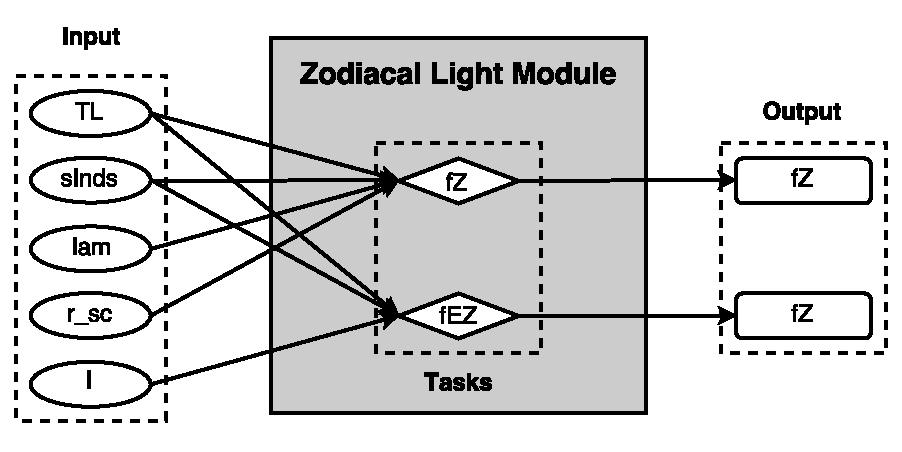
\includegraphics[width=0.8\textwidth]{ZodiTasks}
        \end{tabular}
    \end{center}
    \caption{\label{fig:zodiacallightmodule} Depiction of Zodiacal Light module method including inputs and outputs (see \S\ref{sec:fZtask} and \S\ref{sec:fEZtask}).}
\end{figure}

\subsubsection{Zodiacal Light Object Attribute Initialization}
\subsubsection*{Input}
\begin{itemize}
\item
\begin{description}
    \item
        \item[magZ] \hfill \\
        Zodi brightness magnitude (per $ arcsec^2 $). Defaults to 23.
        \item[magEZ] \hfill \\
        Exo-zodi brightness magnitude (per $ arcsec^2 $). Defaults to 22.
        \item[varEZ] \hfill \\
        Exo-zodiacal light variation (variance of log-normal distribution). Constant if set to 0.  Defaults to 0.
        \item[nEZ] \hfill \\
        Exo-zodiacal light level in zodi. Defaults to 1.5.
\end{description}
\end{itemize}

\subsubsection*{Attributes}
\begin{itemize}
\item
\begin{description}
        \item[magZ (float)] \hfill \\
        Zodi brightness magnitude (per $ arcsec^2 $)
        \item[magEZ (float)] \hfill \\
        Exo-zodi brightness magnitude (per $ arcsec^2 $)
        \item[varEZ (float)] \hfill \\
        Exo-zodiacal light variation (variance of log-normal distribution)
        \item[nEZ (float)] \hfill \\
        Exo-zodiacal light level in zodi
\end{description}
\end{itemize}

\subsubsection{fZ Method} \label{sec:fZtask}
The \verb+fZ+ method returns surface brightness of local zodiacal light for planetary systems.  This functionality is used by the Simulated Universe module.

\subsubsection*{Inputs}
\begin{itemize}
    \item 
    \begin{description}
        \item[TL (object)] \hfill \\ TargetList class object, see \S\ref{sec:targetlist} for description of functionality and attributes       
        \item[sInds (integer ndarray)] \hfill \\ Integer indices of the stars of interest, with the length of the number of planets of interest
        \item[lam (astropy Quantity)] \hfill \\ Central wavelength in units of $ nm $
        \item[r\_sc (astropy Quantity 1$\times$3 array)] \hfill \\ Observatory position vector in units of $ km $
    \end{description}
\end{itemize}
\subsubsection*{Outputs}
\begin{itemize}
    \item 
    \begin{description}
        \item[fZ (astropy Quantity array)] \hfill \\ Surface brightness of zodiacal light in units of $ 1/arcsec^2 $
    \end{description}
\end{itemize}

\subsubsection{fEZ Method} \label{sec:fEZtask}
The \verb+fEZ+ method returns surface brightness of exo-zodiacal light for planetary systems.  This functionality is used by the Simulated Universe module.

\subsubsection*{Inputs}
\begin{itemize}
    \item 
    \begin{description}
        \item[TL (object)] \hfill \\ TargetList class object, see \S\ref{sec:targetlist} for description of functionality and attributes       
        \item[sInds (integer ndarray)] \hfill \\ Integer indices of the stars of interest, with the length of the number of planets of interest
        \item[I (astropy Quantity array)] \hfill \\ Inclination of the planets of interest in units of $ deg $
    \end{description}
\end{itemize}

\subsubsection*{Outputs}
\begin{itemize}
    \item 
    \begin{description}
        \item[fEZ (astropy Quantity array)] \hfill \\
        Surface brightness of exo-zodiacal light in units of $ 1/arcsec^2 $
    \end{description}
\end{itemize}

\subsection{Background Sources}\label{sec:backgroundsources}

The Background Sources module will provide density of background sources for a given target based on its coordinates and the integration depth.  This will be used in the post-processing module to determine false alarms based on confusion.  The prototype module has no inputs and only a single function: \verb+dNbackground+.

\subsubsection{dNbackground}
\subsubsection*{Inputs}
\begin{itemize}
    \item 
    \begin{description}
        \item[coords (astropy SkyCoord array)] \hfill \\ \href{http://astropy.readthedocs.org/en/latest/api/astropy.coordinates.SkyCoord.html}{SkyCoord object} containing right ascension, declination, and  distance to star of the planets of interest in units of $ deg $, $ deg $ and $ pc $.
        \item[intDepths (float ndarray)] \hfill \\ Integration depths equal to absolute magnitudes (in the detection band) of the dark hole to be produced for each target. Must be of same length as coords.
    \end{description}
\end{itemize}
\subsubsection*{Outputs}
\begin{itemize}
    \item 
    \begin{description}
        \item[dN (astropy Quantity array)] \hfill \\
        Number densities of background sources for given targets in  units of $ 1/arcmin^2 $. Same length as inputs.
    \end{description}
\end{itemize}


% OBSERVATORY

\subsection{Observatory}
The Observatory module contains all of the information specific to the space-based observatory not included in the Optical System module. The module has two main methods: \verb+orbit+ and \verb+keepout+, which are implemented as functions within the module. 

The observatory orbit plays a key role in determining which of the target stars may be observed for planet finding at a specific time during the mission lifetime. The Observatory module's \verb+orbit+ method takes the current mission time as input and outputs the observatory's position vector. The position vector is standardized throughout the modules to be referenced to a heliocentric equatorial frame at the J2000 epoch. The observatory's position vector is used in the \verb+keepout+ method and Target List module to determine which of the stars are observable at the current mission time.

The \verb+keepout+ method determines which target stars are observable at a specific time during the mission simulation and which are unobservable due to bright objects within the field of view such as the sun, moon, and solar system planets.  The keepout volume is determined by the specific design of the observatory and, in certain cases, by the starlight suppression system.  The \verb+keepout+ method takes the current mission time and Star Catalog or Target List module output as inputs and outputs a list of the target stars which are observable at the current time. It constructs position vectors of the target stars and bright objects which may interfere with observations with respect to the observatory. These position vectors are used to determine if bright objects are in the field of view for each of the potential stars under exoplanet finding observation.  If there are no bright objects obstructing the view of the target star, it becomes a candidate for observation in the Survey Simulation module.  The solar keepout is typically encoded as allowable angle ranges for the spacecraft-star unit vector as measured from the spacecraft-sun vector.

In addition to these methods, the observatory definition can also encode finite resources used by the observatory throughout the mission.  The most important of these is the fuel used for stationkeeping and repointing, especially in the case of occulters which must move significant distances between observations.  Other considerations could include the use of other volatiles such as cryogens for cooled instruments, which tend to deplete solely as a function of mission time.  This module also allows for detailed investigations of the effects of orbital design on the science yield, e.g., comparing the original baseline geosynchronous 28.5\textdegree{} inclined orbit for WFIRST-AFTA with an L2 halo orbit, which is the new mission baseline. 

The inputs, outputs, and updated attributes of the required Observatory module methods are depicted in  \reffig{fig:observatorymodule}.

\begin{figure}[ht]
    \begin{center}
        \begin{tabular}{c}
             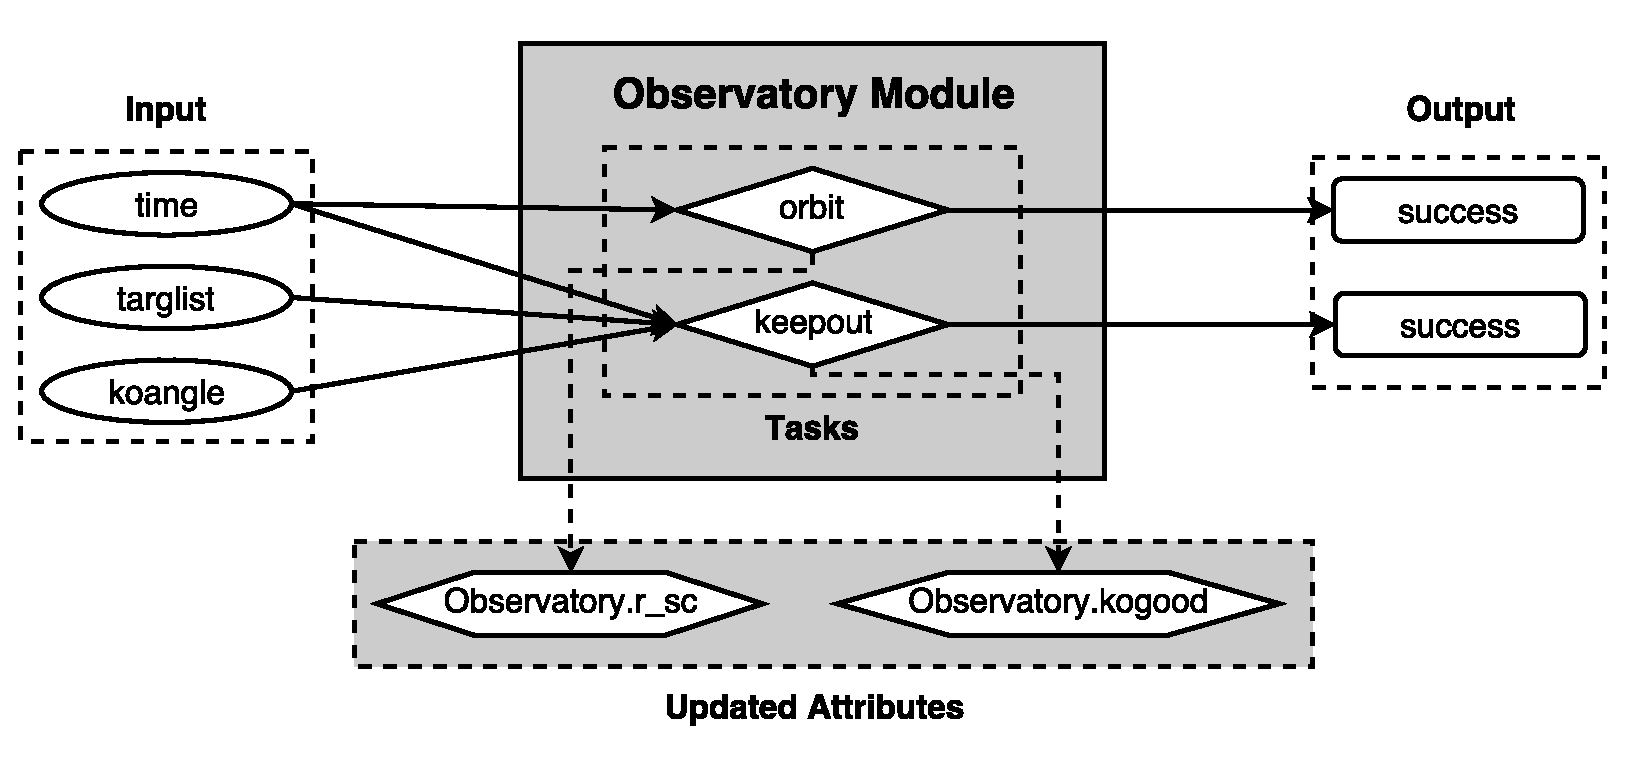
\includegraphics[width=0.9\textwidth]{observatory3}
        \end{tabular}
    \end{center}
    \caption{\label{fig:observatorymodule} Depiction of Observatory module methods including inputs, outputs, and updated attributes (see \S\ref{sec:orbittask} and \S\ref{sec:keepouttask}).}
\end{figure}

\label{sec:observatory}
\subsubsection{Observatory Object Attribute Initialization}

\subsubsection*{Inputs}
\begin{itemize}
    \item
    % \begin{description}
    %     \item[User specification] \hfill \\
    %     Information from simulation specification JSON file organized into a Python dictionary. If the below \verb+key:value+ pairs are missing from the dictionary, the Observatory object attributes will be assigned the default values listed.
        \begin{description}
            \item[settlingTime] \hfill \\
            Amount of time needed for observatory to settle after a repointing in $ day $. Default value is 1.
            \item[thrust] \hfill \\
            Occulter slew thrust in $ mN $. Default value is 450.
            \item[slewIsp] \hfill \\
            Occulter slew specific impulse in $ s $. Default value is 4160.
            \item[scMass] \hfill \\
            Occulter (maneuvering spacecraft) initial wet mass in $ kg $. Default value is 6000.
            \item[dryMass] \hfill \\
            Occulter (maneuvering spacecraft) dry mass in $ kg $. Default value is 3400.
            \item[coMass] \hfill \\
            Telescope (or non-maneuvering spacecraft) mass in $ kg $. Default value is 5800.
            \item[skIsp] \hfill \\
            Specific impulse for station keeping in $ s $. Default value is 220.
            \item[defburnPortion] \hfill \\
            Default burn portion for slewing. Default value is 0.05
            \item[spkpath] \hfill\\
            String with full path to SPK kernel file (only used if using jplephem for solar system body propagation - see \ref{sec:ssbPosTask}.
            \item[forceStaticEphem] \hfill \\
            Boolean, forcing use of static solar system ephemeris if set to True, even if jplephem module is present (see \ref{sec:ssbPosTask}).  Default value is False.
        \end{description}
    % \end{description}
\end{itemize}

\subsubsection*{Attributes}
\begin{itemize}
    \item
    \begin{description}
        \item[settlingTime] \hfill \\
        Amount of time needed for observatory to settle after a repointing (astropy Quantity initially set in $ day $)
        \item[thrust] \hfill \\
        Occulter slew thrust (astropy Quantity initially set in $ mN $)
        \item[slewIsp] \hfill \\
        Occulter slew specific impulse (astropy Quantity initially set in $ s $)
        \item[scMass] \hfill \\
        Occulter (maneuvering spacecraft) initial wet mass (astropy Quantity initially set in $ kg $)
        \item[dryMass] \hfill \\
        Occulter (maneuvering spacecraft) dry mass (astropy Quantity initially set in $ kg $)
        \item[coMass] \hfill \\
        Telescope (or non-maneuvering spacecraft) mass (astropy Quantity initially set in $ kg $)
        \item[kogood] \hfill \\
        1D NumPy ndarray of Boolean values where True is a target unobstructed and observable in the keepout zone. Initialized to an empty array. This attribute is updated to the current mission time through the keepout method (see \ref{sec:keepouttask}).
        \item[r\_sc] \hfill \\
        Observatory orbit position in HE reference frame. Initialized to NumPy ndarray as numpy.array([0., 0., 0.]) and associated with astropy Quantity in $ km $. This attribute is updated to the orbital position of the observatory at the current mission time through the orbit method (see \ref{sec:orbittask}).
        \item[skIsp] \hfill \\
        Specific impulse for station keeping (astropy Quantity initially set in $ s $)
        \item[defburnPortion] \hfill \\
        Default burn portion for slewing
        \item[currentSep] \hfill \\
        Current occulter separation (astropy Quantity initially set in $ km $
        \item[flowRate] \hfill \\
        Slew flow rate derived from thrust and slewIsp (astropy Quantity initially set in $ kg/day $)
        
    \end{description}
\end{itemize}

\subsubsection{orbit Method} \label{sec:orbittask}
The \verb+orbit+ method finds the heliocentric equatorial position vector of the observatory spacecraft.

\subsubsection*{Inputs}
\begin{itemize}
    \item
    \begin{description}
        \item[time] \hfill \\
        astropy \href{http://astropy.readthedocs.org/en/latest/time/index.html}{Time object} which may be \verb+TimeKeeping.currenttimeAbs+ from Time Keeping module see \ref{sec:currenttime} for definition
    \end{description}
\end{itemize}

\subsubsection*{Outputs}
\begin{itemize}
    \item
    \begin{description}
        \item[success] \hfill \\
        Boolean indicating if orbit was successfully calculated
    \end{description}
\end{itemize}

\subsubsection*{Updated Object Attributes}
\begin{itemize}
    \item
    \begin{description}
        \item[Observatory.r\_sc] \hfill \\
        Observatory orbit position in HE reference frame at current mission time (astropy Quantity defined in $ km $)
    \end{description}
\end{itemize}

\subsubsection{keepout Method} \label{sec:keepouttask} 
The \verb+keepout+ method determines which stars in the target list are observable at the given input time.

\subsubsection*{Inputs}
\begin{itemize}
    \item
    \begin{description}
        \item[time] \hfill \\
        astropy Time object which may be \verb+TimeKeeping.currenttimeAbs+ (see \ref{sec:currenttime} for definition)
        \item[targlist] \hfill \\
        Instantiated Target List object from Target List module. See \ref{sec:targetlist} for definition of available attributes
        \item[koangle] \hfill \\
        Telescope keepout angle in $ deg $ - \verb+OpticalSystem.telescopeKeepout+
    \end{description}
\end{itemize}

\subsubsection*{Outputs}
\begin{itemize}
    \item
    \begin{description}
        \item[success] \hfill \\
        Boolean indicating if orbit was successfully calculated
    \end{description}
\end{itemize}

\subsubsection*{Updated Object Attributes}
\begin{itemize}
    \item 
    \begin{description}
        \item[Observatory.kogood] \hfill \\
        1D NumPy ndarray of Boolean values for each target at given time where True is a target unobstructed in the keepout zone and False is a target unobservable due to obstructions in the keepout zone
    \end{description}
\end{itemize}

\subsubsection{solarSystem\_body\_position Method}\label{sec:ssbPosTask}
The \verb+solarSystem_body_position+ returns the position of any solar system body (Earth, Sun, Moon, etc.) at a given time in the common Heliocentric Equatorial frame.  The observatory prototype will attempt to load the jplephem module, and use a local SPK file for all propagations if available.  The SPK file is not packaged with the software but may be downloaded from JPL's website at: \url{http://naif.jpl.nasa.gov/pub/naif/generic_kernels/spk/planets/a_old_versions/}.  The location of the spk file is assumed to be in the Observatory directory but can be set by the \verb+spkpath+ input.  

If jplephem is not present, the Observatory prototype will load static ephemeris derived from Vallado (2004) and use those for propagation.  This behavior can be forced even when jplephem is available by setting the \verb+forceStaticEphem+ input to True.

\subsubsection*{Inputs}
\begin{itemize}
    \item
    \begin{description}
        \item[time] \hfill \\
        astropy Time object which may be \verb+TimeKeeping.currenttimeAbs+ (see \ref{sec:currenttime} for definition)
        \item[bodyname] \hfill \\
        String containing object name, capitalized by convention.
    \end{description}
\end{itemize}

\subsubsection*{Outputs}
\begin{itemize}
    \item
    \begin{description}
        \item[r\_body] \hfill \\
        (Quantity) heliocentric equatorial position vector (units of km)
    \end{description}
\end{itemize}

% TIME KEEPING 

\subsection{Time Keeping} \label{sec:time}
The Time Keeping module is responsible for keeping track of the current mission time.  It encodes only the mission start time, the mission duration, and the current time within a simulation.  All functions in all modules requiring knowledge of the current time call functions or access parameters implemented within the Time module.  Internal encoding of time is implemented as the time from mission start (measured in $ day $).  The Time Keeping module also provides functionality for converting between this time measure and standard measures such as Julian Day Number and UTC time.
  
The Time Keeping module contains the \verb+update_times+ and \verb+duty_cycle+ methods.  These  methods updates the mission time during a survey simulation.  The duty cycle determines when during the mission timeline the observatory is allowed to perform planet-finding operations.  The duty cycle function takes the current mission time as input and outputs the next available time when exoplanet observations may begin or resume, along with the duration of the observational period. The outputs of this method are used in the Survey Simulation module to determine when and how long exoplanet finding and characterization observations occur.  The inputs and updated attributes for the Time Keeping methods are depicted in \reffig{fig:timekeepingmodule}.

\begin{figure}[ht]
    \begin{center}
        \begin{tabular}{c}
             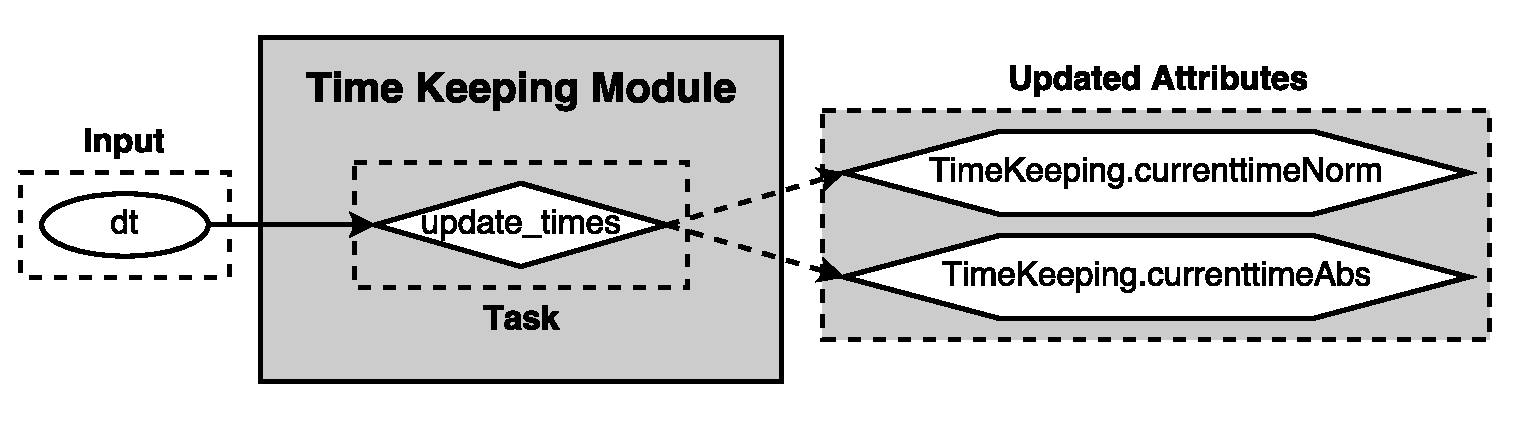
\includegraphics[width=\textwidth]{TimeKeepingTasks}
        \end{tabular}
    \end{center}
    \caption{\label{fig:timekeepingmodule} Depiction of Time Keeping module method including input and updated attributes (see \S\ref{sec:updatetimestask} and \S\ref{sec:dutycycletask}).}
\end{figure}

\subsubsection{Time Keeping Object Attribute Initialization}

\subsubsection*{Inputs}
\begin{itemize}
    \item
     \begin{description}
            \item[missionStart] \hfill \\
            Mission start time in $ MJD $. Default value is 60634.
            \item[missionLife] \hfill \\
            Total length of mission in $ years $. Default value is 6.
            \item[extendedLife] \hfill \\
            Extended mission time in $ years $. Default value is 0.  Extended life typically differs from the primary mission in some way---most typically only revisits are allowed.
            \item[missionPortion] \hfill \\
            Portion of mission time devoted to planet-finding. Default value is 1/6.
        \end{description}
\end{itemize}

\subsubsection*{Attributes}
\begin{itemize}
    \item
    \begin{description}
        \item[missionStart] \hfill \\
        Mission start time (astropy Time object initially defined in $ MJD $)
        \item[missionLife] \hfill \\
        Mission lifetime (astropy Quantity initially set in $ years $)
        \item[extendedLife] \hfill \\
        Extended mission time (astropy Quantity initially set in $ years $)
        \item[missionPortion] \hfill \\
        Portion of mission time devoted to planet-finding
        \item[duration] \hfill \\
        Duration of planet-finding operations (astropy Quantity initially set in $ day $)
        \item[nexttimeAvail] \hfill \\
        Next time available for planet-finding (astropy Quantity initially set in $ day $)
        \item[currenttimeNorm] \hfill \\
        Current mission time normalized so that start date is 0 (astropy Quantity initially set in $ day $)
        \item[currenttimeAbs] \label{sec:currenttime}\hfill \\
        Current absolute mission time (astropy Time object initially defined in $ MJD $)
        \item[missionFinishNorm] \hfill \\
        Mission finish time (astropy Quantity initially set in $ day $)
        \item[missionFinishAbs] \hfill \\
        Mission completion date (astropy Time object initially defined in $ MJD $)
    \end{description}
\end{itemize}

\subsubsection{update\_times Method} \label{sec:updatetimestask}
The \verb+update_times+ method updates the relevant mission times.

\subsubsection*{Inputs}
\begin{itemize}
    \item 
    \begin{description}
        \item[dt] \hfill \\
        Time increment (astropy Quantity with units of time)
    \end{description}
\end{itemize}

\subsubsection*{Updated Object Attributes}
\begin{itemize}
    \item 
    \begin{description}
        \item[TimeKeeping.currenttimeNorm] \hfill \\
        Current mission time normalized so that start date is 0 (astropy Quantity with units of time)
        \item[TimeKeeping.currenttimeAbs] \hfill \\
        Current absolute mission time (astropy Time object)
    \end{description}
\end{itemize}

\subsubsection{duty\_cycle Method} \label{sec:dutycycletask}
The \verb+duty_cycle+ method calculates the next time that the observatory will be available for exoplanet science and returns this time and the maximum amount of time afterwards during which an exolanet observation can run (if capped).

\subsubsection*{Inputs}
\begin{itemize}
    \item 
    \begin{description}
        \item[currenttime] \hfill \\
        Current time in mission simulation (astropy Quantity with units of time often \verb+TimeKeeping.currenttimeNorm+)
    \end{description}
\end{itemize}

\subsubsection*{Outputs}
\begin{itemize}
    \item 
    \begin{description}
        \item[nexttime] \hfill \\
        Next available time for planet-finding (astropy Quantity with units of time)
    \end{description}
\end{itemize}

\subsubsection*{Updated Object Attributes}
\begin{itemize}
    \item 
    \begin{description}
        \item[TimeKeeping.nexttimeAvail] \hfill \\
        Next time available for planet-finding (astropy Quantity with units of time)
        \item[TimeKeeping.duration] \hfill \\
        Duration of planet-finding operations (astropy Quantity with units of time)
    \end{description}
\end{itemize}

% POST-PROCESSING

\subsection{Post-Processing}\label{sec:postprocessing}
The Post-Processing module encodes the effects of post-processing on the data gathered in a simulated observation, and the effects on the final contrast of the simulation.  The Post-Processing module is also responsible for determining whether a planet detection has occurred for a given observation, returning one of four possible states---true positive (real detection), false positive (false alarm), true negative (no detection when no planet is present) and false negative (missed detection).  These can be generated based solely on statistical modeling or by processing simulated images.

The Post-Processing module contains the \verb+det_occur+ task.  This task determines if a planet detection occurs for a given observation.  The inputs and outputs for this task are depicted in \reffig{fig:postprocessingmodule}.

\begin{figure}[ht]
    \begin{center}
        \begin{tabular}{c}
             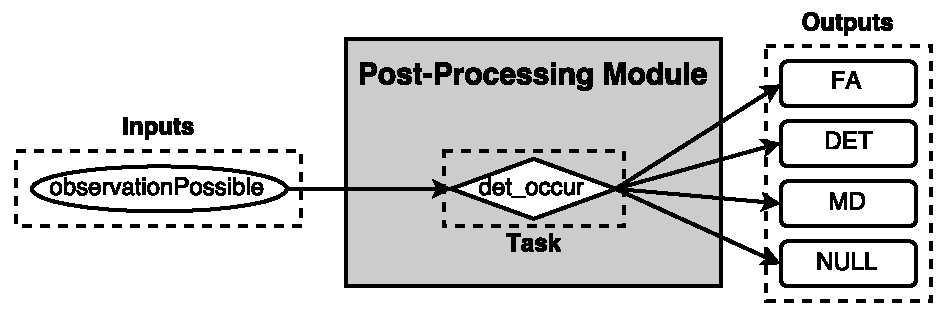
\includegraphics[width=0.8\textwidth]{PostTasks}
        \end{tabular}
    \end{center}
    \caption{\label{fig:postprocessingmodule} Depiction of Post-Processing module task including inputs and outputs (see \S\ref{sec:detoccurtask}).}
\end{figure}

\subsubsection{Post-Processing Object Attribute Initialization}
\subsubsection*{Inputs}
\begin{itemize}
    \item 
    \begin{description}
          \item[FAP] \hfill \\
            Detection false alarm probability. Default value is $3 \times 10^{-5}$.
            \item[MDP] \hfill \\
            Missed detection probability. Default value is $10^{-3}$.
            \item[ppFact] \hfill \\
            Post-processing contrast factor, between 0 and 1. Default value is 1.
            \item[SNimag] \hfill \\
            Signal to Noise Ratio threshold for imaging/detection. Default value is 5.
            \item[SNchar] \hfill \\
            Signal to Noise Ratio threshold for characterization. Default value is 11.
        \end{description}
\end{itemize}

\subsubsection*{Attributes}
\begin{itemize}
    \item 
    \begin{description}
        \item[BackgroundSources (object)] \hfill \\
        BackgroundSources class object (see \ref{sec:backgroundsources})
        \item[FAP] \hfill \\
        Detection false alarm probability
        \item[MDP] \hfill \\
        Missed detection probability
    \end{description}
\end{itemize}

\subsubsection{det\_occur Method} \label{sec:detoccurtask}
The \verb+det_occur+ method determines if a planet detection has occurred.

\subsubsection*{Inputs}
\begin{itemize}
    \item 
    \begin{description}
        \item[observationPossible] \hfill \\
        1D NumPy ndarray of booleans signifying if a planet in the system being observed is observable
    \end{description}
\end{itemize}

\subsubsection*{Outputs}
\begin{itemize}
    \item 
    \begin{description}
        \item[FA] \hfill \\
        Boolean where True means False Alarm
        \item[DET] \hfill \\
        Boolean where True means DETection
        \item[MD] \hfill \\
        Boolean where True means Missed Detection
        \item[NULL] \hfill \\
        Boolean where True means Null Detection
    \end{description}
\end{itemize}


% COMPLETENESS

\subsection{Completeness}\label{sec:completeness}
The Completeness module takes in information from the Planet Population module to determine initial completeness and update completeness values for target list stars when called upon.

The Completeness module contains the following methods: \verb+target_completeness+ and \verb+completeness_update+. \verb+target_completeness+ generates initial completeness values for each star in the target list (see \S\ref{sec:targetcompletenesstask}). \verb+completeness_update+ updates the completeness values following an observation (see \S\ref{sec:completenessupdatetask}).

\subsubsection{Completeness Object Attribute Initialization}

\subsubsection*{Input}
Monte Carlo methods for calculating completeness will require an input of the number of planet samples called \verb+Nplanets+. 


\subsubsection*{Attributes}
\begin{itemize}
    \item 
    \begin{description}
        \item[PlanetPopulation] \hfill \\
        Planet Population module object (see \ref{sec:planetpopulation})
        \item[PlanetPhysicalModel] \hfill \\
        Planet Physical Model module object (see \ref{sec:planetphysicalmodel}) 
    \end{description}
\end{itemize}

\subsubsection{target\_completeness Method}
\label{sec:targetcompletenesstask}
The \verb+target_completeness+ method generates completeness values for each star in the target list.

\subsubsection*{Inputs}
\begin{itemize}
    \item 
    \begin{description}
        \item[targlist] \hfill \\
        Instantiated Target List object from Target List module see \S\ref{sec:targetlist} for definition of functionality and attributes
    \end{description}
\end{itemize}

\subsubsection*{Outputs}
\begin{itemize}
    \item 
    \begin{description}
        \item[comp0] \hfill \\
        1D NumPy ndarray containing completeness values for each star in the target list
    \end{description}
\end{itemize}

\subsubsection{gen\_update Method} \label{sec:genupdatetask}
The \verb+gen_update+ method generates dynamic completeness values for successive observations of each star in the target list.

\subsubsection*{Input}
\begin{itemize}
    \item 
    \begin{description}
            \item[TL] \hfill \\
            Instantiated Target List object from Target List module see \S\ref{sec:targetlist} for definition of functionality and attributes
    \end{description}
\end{itemize}

\subsubsection{completeness\_update Method}
\label{sec:completenessupdatetask}
The \verb+completeness_update+ method updates the completeness values for each star in the target list following an observation.

\subsubsection*{Inputs}
\begin{itemize}
    \item 
    \begin{description}
        \item[s\_ind] \hfill \\
        index of star in target list just observed
        \item[targlist] \hfill \\
        Instantiated Target List object from Target List module see \S\ref{sec:targetlist} for definition of functionality and attributes
        \item[obsbegin] \hfill \\
        Mission time when the observation of \verb+s_ind+ began (astropy Quantity with units of time)
        \item[obsend] \hfill \\
        Mission time when the observation of \verb+s_ind+ ended (astropy Quantity with units of time)
        \item[nexttime] \hfill \\
        Mission time of next observational period (astropy Quantity with units of time)
    \end{description}
\end{itemize}

\subsubsection*{Output}
\begin{itemize}
    \item 
    \begin{description}
        \item[comp0] \hfill \\
        1D NumPy ndarray of updated completeness values for each star in the target list
    \end{description}
\end{itemize}

% TARGET LIST

\subsection{Target List}
The Target List module takes in information from the Optical System, Star Catalog, Planet Population, and Observatory modules and Completeness module to generate the target list for the simulated survey.  This list can either contain all of the targets where a planet with specified parameter ranges could be observed or a list of pre-determined targets such as in the case of a mission which only seeks to observe stars where planets are known to exist from previous surveys.  The final target list encodes all of the same information as is provided by the Star Catalog module.

\label{sec:targetlist}
\subsubsection{Target List Object Attribute Initialization}
\subsubsection*{Inputs}
\begin{itemize}
    \item 
    \begin{description}
        % \item[User specification] \hfill \\
        % Information from simulation specification JSON file organized into a Python dictionary. If \verb+key:value+ pairs are missing from the dictionary, the Target List object attributes will be assigned the default values.
        \item[keepStarCatalog] \hfill \\
        Boolean representing whether to delete the star catalog object after the target list is assembled (defaults to False).  If True, object reference will be available from TargetList class object.
        \item[minComp] \hfill \\
        Minimum completeness value for inclusion in target list.  Defaults to 0.1.
    \end{description}
\end{itemize}

\subsubsection*{Attributes}
\begin{itemize}
    \item 
    \begin{description}
        \item[(StarCatalog values)] \hfill \\
        Mission specific filtered star catalog values from StarCatalog class object (see \ref{sec:starcatalog})
        \item[PlanetPopulation (object)] \hfill \\
        PlanetPopulation class object (see \ref{sec:planetpopulation})
        \item[PlanetPhysicalModel (object)] \hfill \\
        PlanetPhysicalModel class object (see \ref{sec:planetphysicalmodel})
        \item[StarCatalog (object)]\hfill \\
        StarCatalog class object (only retained if keepStarCatalog is True, see \ref{sec:starcatalog})
        \item[OpticalSystem (object)] \hfill \\
        OpticalSystem class object (see \ref{sec:opticalsystem})
        \item[ZodiacalLight (object)] \hfill \\
        ZodiacalLight class object (see \ref{sec:zodiacallight})
        \item[BackgroundSources (object)] \hfill \\
        BackgroundSources class object (see \ref{sec:backgroundsources})
        \item[PostProcessing (object)] \hfill \\
        PostProcessing class object (see \ref{sec:postprocessing})
        \item[Completeness (object)] \hfill \\
        Completeness class object (see \ref{sec:completeness})
        \item[maxintTime (astropy Quantity array)] \hfill \\
        Maximum integration time for each target star in units of $ day $. Calculated from \verb+OpticalSystem.calc_maxintTime+ \S\ref{sec:calcmaxintTimetask}
        \item[comp0 (float ndarray)] \hfill \\
        Completeness value for each target star. Calculated from \verb+Completeness.target_completeness+ \S\ref{sec:targetcompletenesstask}
        \item[minComp (float)] \hfill \\
        Minimum completeness value for inclusion in target list. 
        \item[MsEst (float ndarray)] \hfill \\
        Approximate stellar mass in $ M_{sun} $
        \item[MsTrue (float ndarray)] \hfill \\
        Stellar mass with an error component included in $ M_{sun} $
        \item[nStars (int)] \hfill \\
        Number of target stars
    \end{description}
\end{itemize}

\subsubsection{starMag Method} \label{sec:starMagtask}
The \verb+starMag+ method calculates star visual magnitudes with B-V color using empirical fit to data from Pecaut and Mamajek (2013, Appendix C). The expression for flux is accurate to about $7\%$, in the range of validity 400 $ nm < \lambda < $ 1000 $ nm $ (Traub et al. 2016).
\subsubsection*{Inputs}
\begin{itemize}
    \item 
    \begin{description}
        \item[sInds (integer ndarray)] \hfill \\
        Indices of the stars of interest, with the length of the number 
        of planets of interest
        \item[lam (astropy Quantity)] \hfill \\
        Wavelength in units of $ nm $
    \end{description}
\end{itemize}
\subsubsection*{Output}
\begin{itemize}
    \item
    \begin{description}
        \item[mV (float ndarray)] \hfill \\
        Star visual magnitudes with B-V color
    \end{description}
\end{itemize}

\subsubsection{populate\_target\_list method} \label{sec:populatetargetlisttask}

This method is responsible for populating values from the star catalog  (or any other source) into the target list attributes. It has not specific inputs and outputs, but is always passed the full specification dictionary, and updates all relevant Target List attributes.  This method is called from the prototype constructor, and does not need to be called from the implementation constructor when overloaded in the implementation.   The prototype implementation copies values directly from star catalog and removes stars with any NaN attributes. It also calls the \verb+target_completeness+ in the Completeness module (\S\ref{sec:targetcompletenesstask}) and the \verb+calc_maxintTime+ in the Optical System module (\S\ref{sec:calcmaxintTimetask}) to generate the initial completeness and maximum integration time for all targets.  It also generates 'true' and 'approximate' star masses using object method \verb+stellar_mass+ (see below).

\subsubsection{filter\_target\_list method}  \label{sec:filtertargetlisttask}
This method is responsible for filtering the targetlist to produce the values from the star catalog  (or any other source) into the target list attributes. It has not specific inputs and outputs, but is always passed the full specification dictionary, and updates all relevant Target List attributes.  This method is called from the prototype constructor, immediately after the \verb+populate_target_list+ call, and does not need to be called from the implementation constructor when overloaded in the implementation.   The prototype implementation filters out any targets where the widest separation planet in the modeled population would be inside the system IWA, any targets where the limiting delta mag is above the population maximum delta mag, where the integration time for the brightest planet in the modeled population is above the specified maximum integration time, and all targets where the initial completeness is below the specified threshold. 

\subsubsection{Target List Filtering Helper Methods}

The \verb+filter_target_list+ method calls multiple helper functions to perform the actual filtering tasks.  Additional filters can be defined in specific implementations and by overloading the  \verb+filter_target_list+ method.  The filter subtasks (with a few exception) take no inputs and operate directly on object attributes. The prototype implementation implements the following methods:
\begin{itemize}
\item \verb+nan_filter+: Filters any target list entires with NaN values
\item \verb+binary_filter+: Filters any targets with attribute \verb+Binary_Cut+ set to True
\item \verb+main_sequence_filter+: Filters any target lists that are not on the Main Sequence (estimated from the MV and BV attributes)
\item \verb+ fgk_filter+: Filters any targets that are not F, G, or K stars
\item \verb+vis_mag_filter+: Filters out targets with visible magnitudes below input value \verb+Vmagcrit+
\item \verb+outside_IWA_filter+: Filters out targets with all planets inside of the IWA
\item \verb+int_cutoff_filter+: Filters out all targets with maximum integration times above the specified (in the input spec) threshold integration time
\item \verb+max_dmag_filter+: Filters out all targets with minimum delta mag above the limiting delta mag (from input spec)
\item \verb+completeness_filter+: Filters out all targets with single visit completeness below the specified (in the input spec) threshold completeness
\item \verb+revise_lists+: General helper function for applying filters.
\end{itemize}


% SIMULATED UNIVERSE 

\subsection{Simulated Universe} \label{sec:simulateduniverse}
The Simulated Universe module instantiates the Target List module and creates a synthetic universe by populating planetary systems about some or all of the stars in the target list.  For each target, a planetary system is generated based on the statistics encoded in the Planet Population module, so that the overall planet occurrence and multiplicity rates are consistent with the provided distribution functions.  Physical parameters for each planet are similarly sampled from the input density functions (or calculated via the Planet physical model).  All planetary orbital and physical parameters are encoded as arrays of values, with an indexing array that maps planets to the stars in the target list. 

The Simulated Universe module contains the following methods: 
\begin{itemize}
\item[] \verb+gen_planetary_systems+
\item[] \verb+planet_pos_vel+
\item[] \verb+prop_system+
\item[] \verb+get_current_WA+
\end{itemize}

\verb+gen_planetary_systems+ populates the orbital elements and physical characteristics of all planets (see \S\ref{sec:genplanetarysystemstask}). 
\verb+planet_pos_vel+ finds initial position and velocity vectors for each planet (see \S\ref{sec:planetposveltask}).
\verb+prop_system+ propagates planet position,  velocity, and star separation in time (see \S\ref{sec:propsystemtask}).
\verb+get_current_WA+ calculates planet current working angle (see \S\ref{sec:getcurrentWAtask}).
All planetary parameters are generated in the constructor via calls to the appropriate value generating functions in the planet population module.

%\begin{figure}[ht]
%    \begin{center}
%        \begin{tabular}{c}
%             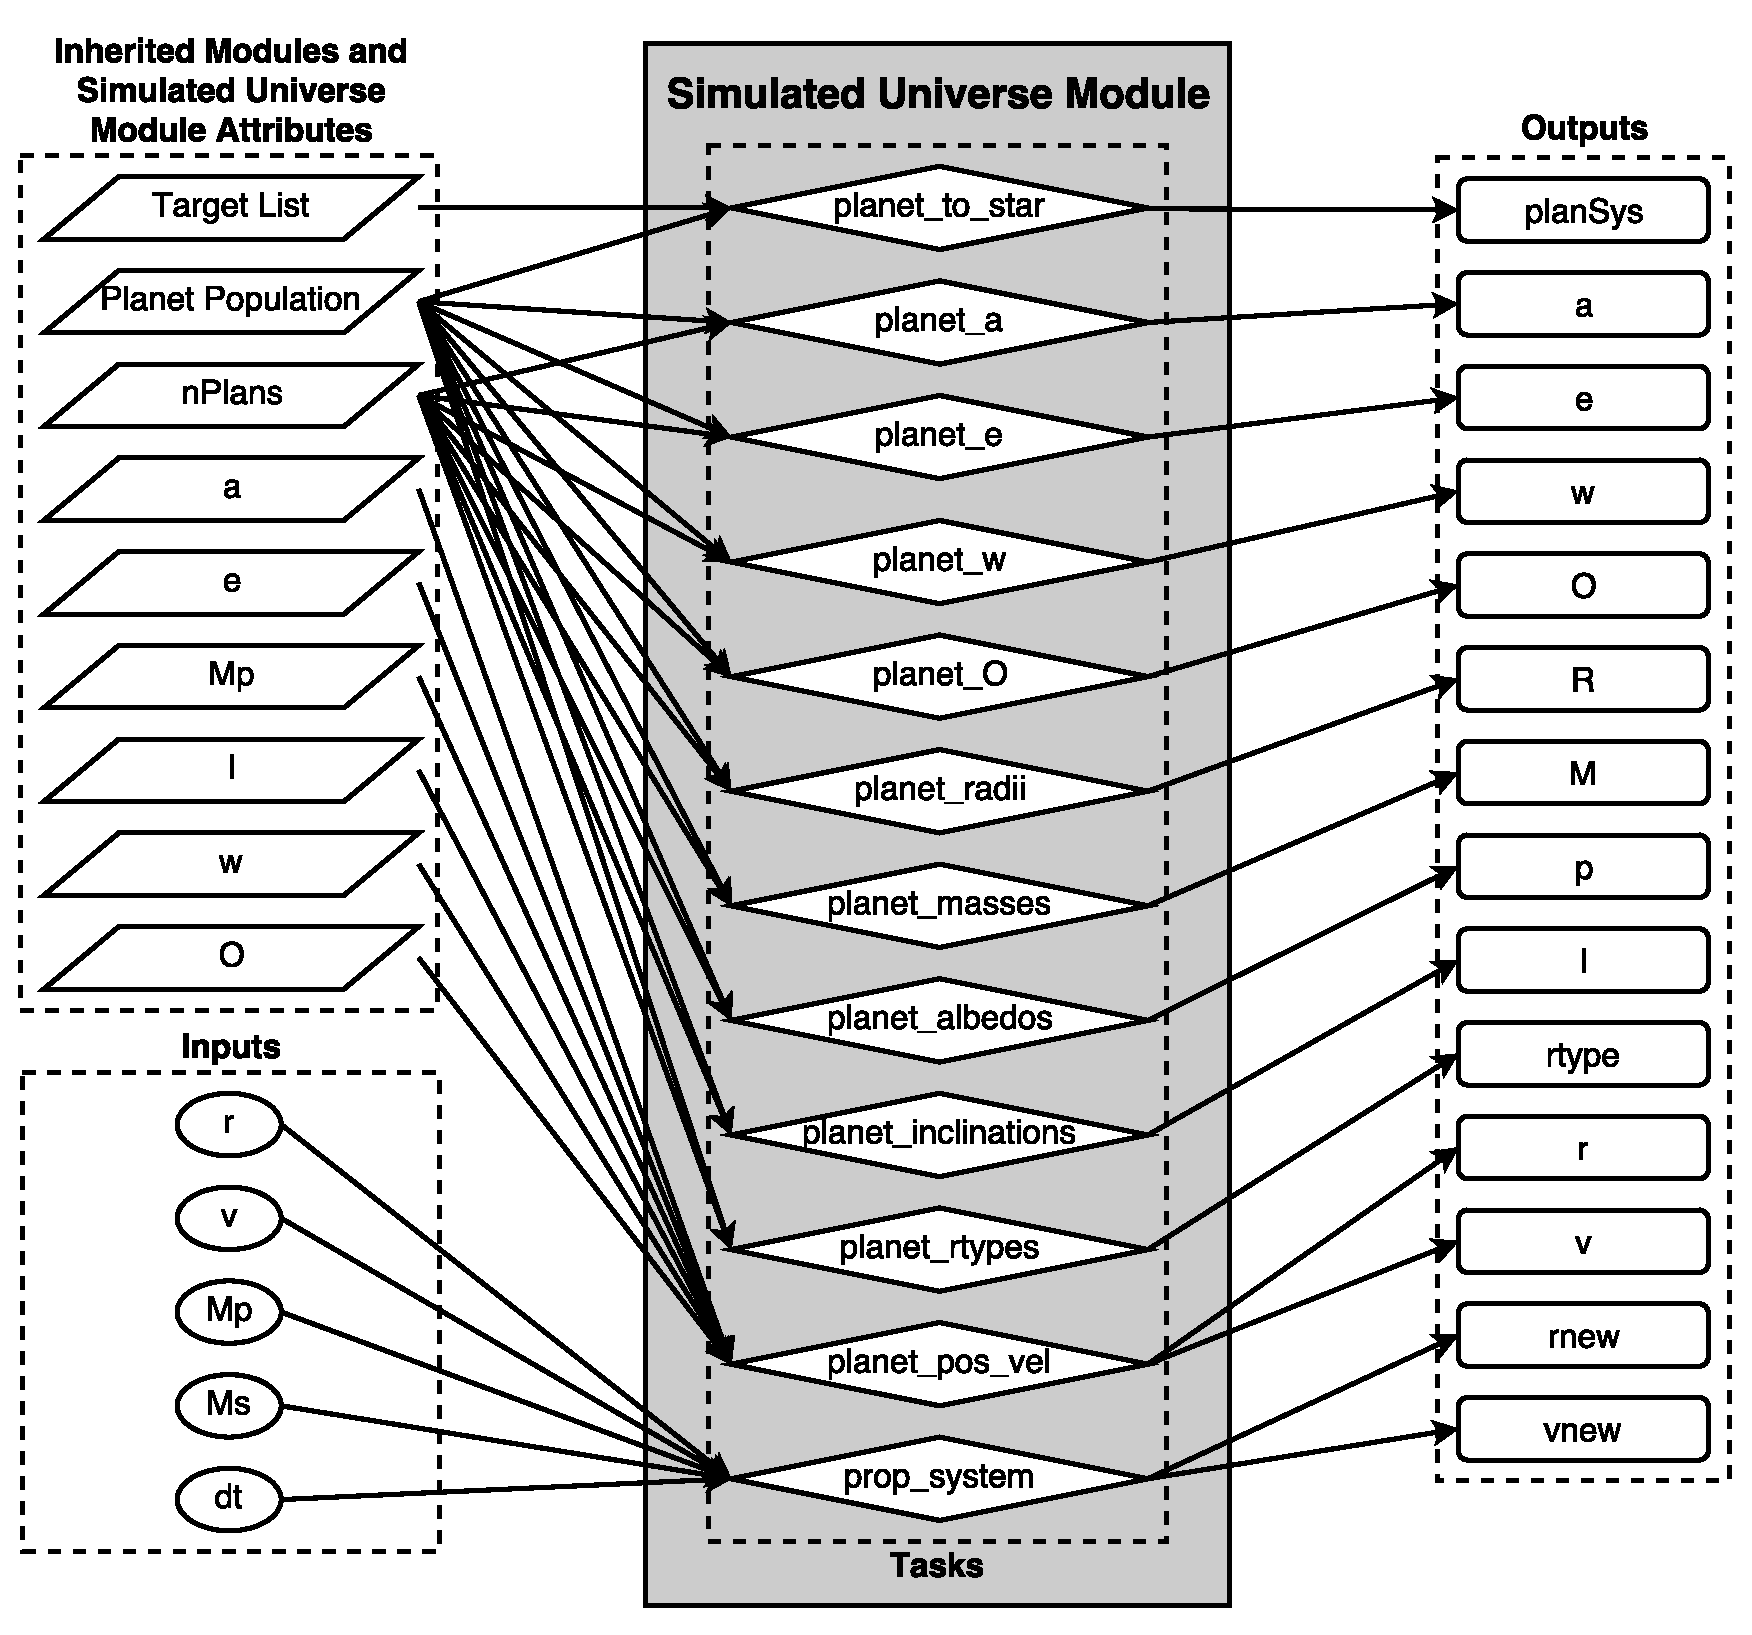
\includegraphics[width=\textwidth]{SimulatedUniverseTasks}
%        \end{tabular}
%    \end{center}
%    \caption{\label{fig:simulateduniversemodule} Depiction of Simulated Universe module methods including inputs and outputs (see \ref{sec:planettostartask}, \ref{sec:planetatask}, \ref{sec:planetetask}, \ref{sec:planetwtask}, \ref{sec:planetOtask}, \ref{sec:planetmassestask}, \ref{sec:planetradiitask}, \ref{sec:planetposveltask}, \ref{sec:planetalbedostask}, \ref{sec:planetinclinationstask}, and \ref{sec:propsystemtask}).}
%\end{figure}

\subsubsection{Attributes}
\begin{itemize}
    \item
    \begin{description}
        \item[PlanetPopulation (object)] \hfill \\
        PlanetPopulation class object (see \ref{sec:planetpopulation})
        \item[PlanetPhysicalModel (object)] \hfill \\
        PlanetPhysicalModel class object (see \ref{sec:planetphysicalmodel})
        \item[OpticalSystem (object)] \hfill \\
        OpticalSystem class object (see \ref{sec:opticalsystem})
        \item[ZodiacalLight (object)] \hfill \\
        ZodiacalLight class object (see \ref{sec:zodiacallight})
        \item[BackgroundSources (object)] \hfill \\
        BackgroundSources class object (see \ref{sec:backgroundsources})
        \item[PostProcessing (object)] \hfill \\
        PostProcessing class object (see \ref{sec:postprocessing})
        \item[Completeness (object)] \hfill \\
        Completeness class object (see \ref{sec:completeness})
        \item[TargetList (object)] \hfill \\
        TargetList class object (see \ref{sec:targetlist})
        \item[eta (float)] \hfill \\
        Global occurrence rate defined as expected number of planets per star in a given universe
        \item[nPlans (integer)] \hfill \\
        Total number of planets
        \item[plan2star (integer ndarray)] \hfill \\
        Indices mapping planets to target stars in TargetList
        \item[sInds (integer ndarray)] \hfill \\
        Unique indices of stars with planets in TargetList
        \item[a (astropy Quantity array)] \hfill \\
        Planet semi-major axis in units of $ AU $
        \item[e (float ndarray)] \hfill \\
        Planet eccentricity
        \item[I (astropy Quantity array)] \hfill \\
        Planet inclination in units of $ deg $ 
        \item[O (astropy Quantity array)] \hfill \\
        Planet right ascension of the ascending node in units of $ deg $
        \item[w (astropy Quantity array)] \hfill \\
        Planet argument of perigee in units of $ deg $
        \item[p (float ndarray)] \hfill \\
            Planet albedo
        \item[Rp (astropy Quantity array)] \hfill \\
            Planet radius in units of $ km $
        \item[Mp (astropy Quantity array)] \hfill \\
            Planet mass in units of $ kg $
        \item[r (astropy Quantity n$\times$3 array)] \hfill \\ Planet position vector in units of $ km $
        \item[v (astropy Quantity n$\times$3 array)] \hfill \\ Planet velocity vector in units of $ km/s $
        \item[s (astropy Quantity array)] \hfill \\
        Planet-star apparent separations in units of $ km $
        \item[d (astropy Quantity array)] \hfill \\
        Planet-star distances in units of $ km $
        \item[fEZ (astropy Quantity array)] \hfill \\
            Surface brightness of exozodiacal light in units of $ 1/arcsec2 $, determined from \verb+ZodiacalLight.fEZ+ \S\ref{sec:fEZtask}
    \end{description}
\end{itemize}

\subsubsection{gen\_planetary\_system Method} \label{sec:genplanetarysystemstask}
The \verb+gen_planetary_system+ method generates the planetary systems for the current simulated universe. This routine populates arrays of the orbital elements and physical characteristics of all planets, and generates indexes that map from planet to parent star.

\subsubsection*{Inputs}
This method does not take any explicit inputs.  It uses the inherited TargetList and PlanetPopulation objects.
\begin{itemize}
    \item 
    \begin{description}
        \item[M (ndarray)] \hfill \\
        Initial mean anomaly of all planets.  Must be an ndarray of the same size as PlanetPopulation.a (and all other orbital parameters).  Must be in radians, in range of $[0,2\pi)$. If set to None (the default) this array will be populated with uniformly distributed random values in that range.
  \end{description}
\end{itemize}

\subsubsection*{Updated Attributes}
\begin{itemize}
    \item 
    \begin{description}
        \item[nPlans (integer)] \hfill \\
        Total number of planets
        \item[plan2star (integer ndarray)] \hfill \\
        Indices mapping planets to target stars in TargetList
        \item[sInds (integer ndarray)] \hfill \\
        Unique indices of stars with planets in TargetList
        \item[a (astropy Quantity array)] \hfill \\
        Planet semi-major axis in units of $ AU $
        \item[e (float ndarray)] \hfill \\
        Planet eccentricity
        \item[I (astropy Quantity array)] \hfill \\
        Planet inclination in units of $ deg $ 
        \item[O (astropy Quantity array)] \hfill \\
        Planet right ascension of the ascending node in units of $ deg $
        \item[w (astropy Quantity array)] \hfill \\
        Planet argument of perigee in units of $ deg $
        \item[r (astropy Quantity n$\times$3 array)] \hfill \\ Planet position vector in units of $ km $
        \item[v (astropy Quantity n$\times$3 array)] \hfill \\ Planet velocity vector in units of $ km/s $
        \item[s (astropy Quantity array)] \hfill \\
        Planet-star apparent separations in units of $ km $
        \item[d (astropy Quantity array)] \hfill \\
        Planet-star distances in units of $ km $
        \item[Mp (astropy Quantity array)] \hfill \\
            Planet mass in units of $ kg $
        \item[Rp (astropy Quantity array)] \hfill \\
            Planet radius in units of $ km $
        \item[p (float ndarray)] \hfill \\
            Planet albedo
        \item[fEZ (astropy Quantity array)] \hfill \\
            Surface brightness of exozodiacal light in units of $ 1/arcsec2 $, determined from \verb+ZodiacalLight.fEZ+ \S\ref{sec:fEZtask}
    \end{description}
\end{itemize}

\subsubsection{planet\_pos\_vel Method} \label{sec:planetposveltask}
The \verb+planet_pos_vel+ method assigns each planet an initial position and velocity vector with appropriate astropy Quantity units attached.

\subsubsection*{Inputs}
This method does not take any explicit inputs.  It uses the following attributes assigned before calling this method:
\begin{itemize}
    \item \verb+SimulatedUniverse.a+
    \item \verb+SimulatedUniverse.e+
    \item \verb+SimulatedUniverse.I+
    \item \verb+SimulatedUniverse.O+
    \item \verb+SimulatedUniverse.w+
    \item \verb+SimulatedUniverse.Mp+
\end{itemize}
\subsubsection*{Outputs}
\begin{itemize}
    \item 
    \begin{description}
        \item[r (astropy Quantity n$\times$3 array)] \hfill \\ Planet position vector in units of $ km $
        \item[v (astropy Quantity n$\times$3 array)] \hfill \\ Planet velocity vector in units of $ km/s $
    \end{description}
\end{itemize}

\subsubsection{prop\_system Method} \label{sec:propsystemtask}
The \verb+prop_system+ method propagates planet state vectors (position and velocity) in time.

\subsubsection*{Inputs}
\begin{itemize}
    \item 
    \begin{description}
        \item[r (astropy Quantity n$\times$3 array)] \hfill \\ Initial position vector of each planet in units of $ km $
        \item[v (astropy Quantity n$\times$3 array)] \hfill \\ Initial velocity vector of each planet in units of $ km/s $
        \item[Mp (astropy Quantity array)] \hfill \\ Planet masses in units of $ kg $
        \item[Ms (float ndarray)] \hfill \\ Target star masses in M\_sun
        \item[dt (astropy Quantity)] \hfill \\ Time increment to propagate the system in units of $ day $
    \end{description}
\end{itemize}
\subsubsection*{Outputs}
\begin{itemize}
    \item 
    \begin{description}
       \item[rnew (astropy Quantity n$\times$3 array)] \hfill \\ Propagated position vectors in units of $ km $
       \item[vnew (astropy Quantity n$\times$3 array)] \hfill \\ Propagated velocity vectors in units of $ km/s $
       \item[snew (astropy Quantity array)] \hfill \\ Propagated apparent separations in units of $ km $
       \item[dnew (astropy Quantity array)] \hfill \\ Propagated planet-star distances in units of $ km $
    \end{description}
\end{itemize}

\subsubsection{get\_current\_WA Method} \label{sec:getcurrentWAtask}
The \verb+get_current_WA+ method calculates the current working angles for planets specified by the given indices.

\subsubsection*{Inputs}
\begin{itemize}
    \item 
    \begin{description}
        \item[pInds (integer ndarray)] \hfill \\
        Integer indices of the planets of interest
    \end{description}
\end{itemize}
\subsubsection*{Outputs}
\begin{itemize}
    \item 
    \begin{description}
        \item[WA (astropy Quantity array)] \hfill \\
        Working angles in units of $ arcsec $
    \end{description}
\end{itemize}

% SURVEY SIMULATION

\subsection{Survey Simulation} \label{sec:surveysim}
The Survey Simulation module takes as input instances of the Simulated Universe  module and the Time Keeping, and Post-Processing modules. This is the module that performs a specific simulation based on all of the input parameters and models. This module returns the mission timeline - an ordered list of simulated observations of various targets on the target list along with their outcomes.  The output also includes an encoding of the final state of the simulated universe (so that a subsequent simulation can start from where a previous simulation left off) and the final state of the observatory definition (so that post-simulation analysis can determine the percentage of volatiles expended, and other engineering metrics).

Survey Simulation TASKS: 
\verb+run_sim()+ - perform survey simulation \S\ref{sec:runsimtask}

Survey Simulation SUBTASKS:
\verb+initial_target()+ - find initial target star \S\ref{sec:initialtargettask}

\verb+observation_detection(pInds, s_ind, DRM, planPosTime)+ - finds if planet detections are possible and returns relevant information \S\ref{sec:observationdetectiontask}\\
\verb+det_data(s, dMag, Ip, DRM, FA, DET, MD, s_ind, pInds, observationPossible, observed)+ - determines detection status \S\ref{sec:detdatatask}
\begin{verbatim}
observation_characterization(observationPossible, pInds, s_ind, spectra,\
	 					s, Ip, DRM, FA, t_int)
\end{verbatim} 
finds if characterizations are possible and returns relevant information \S\ref{sec:observationcharacterizationtask}\\
\verb+next_target(s_ind, revisit_list, extended_list, DRM)+ - find next target (scheduler) \S\ref{sec:nexttargettask}

\subsubsection{Survey Simulation Object Attribute Initialization}
\subsubsection*{Inputs}
\begin{itemize}
    \item 
    \begin{description}
        % \item[User specification] \hfill \\
        % Information from simulation specification JSON file organized into a Python dictionary. If the below \verb+key:value+ pairs are missing from the dictionary, the Survey Simulation object attributes will be assigned the default values listed.
        \item[OpticalSystem] \hfill \\
        Instance of Optical System module inherited from Simulated Universe module (see \ref{sec:opticalsystem})
        \item[PlanetPopulation] \hfill \\
        Instance of Planet Population module inherited from Simulated Universe module (see \ref{sec:planetpopulation})
        \item[ZodiacalLight] \hfill \\
        Instance of Zodiacal Light module inherited from Simulated Universe module (see \ref{sec:zodiacallight})
        \item[Completeness] \hfill \\
        Instance of Completeness module inherited from Simulated Universe module (see \ref{sec:completeness})
        \item[TargetList] \hfill \\
        Instance of Target List module inherited from Simulated Universe module (see \ref{sec:targetlist})
        \item[PlanetPhysicalModel] \hfill \\
        Instance of Planet Physical Model module inherited from Simulated Universe module (see \ref{sec:planetphysicalmodel})
        \item[SimulatedUniverse] \hfill \\
        Instance of Simulated Universe module (see \ref{sec:simulateduniverse})
        \item[Observatory] \hfill \\
        Instance of Observatory module (see \ref{sec:observatory})
        \item[TimeKeeping] \hfill \\
        Instance of Time Keeping module (see \ref{sec:time})
        \item[PostProcessing] \hfill \\
        Instance of Post-Processing module (see \ref{sec:postprocessing})
    \end{description}
\end{itemize}

\subsubsection*{Attributes}
\begin{itemize}
    \item
    \begin{description}
        \item[OpticalSystem] \hfill \\
        Instance of Optical System module (see \ref{sec:opticalsystem})
        \item[PlanetPopulation] \hfill \\
        Instance of Planet Population module (see \ref{sec:planetpopulation})
        \item[ZodiacalLight] \hfill \\
        Instance of Zodiacal Light module (see \ref{sec:zodiacallight})
        \item[Completeness] \hfill \\
        Instance of Completeness module (see \ref{sec:completeness})
        \item[TargetList] \hfill \\
        Instance of Target List module (see \ref{sec:targetlist})
        \item[PlanetPhysicalModel] \hfill \\
        Instance of Planet Physical Model module (see \ref{sec:planetphysicalmodel})
        \item[SimulatedUniverse] \hfill \\
        Instance of Simulated Universe module (see \ref{sec:simulateduniverse})
        \item[Observatory] \hfill \\
        Instance of Observatory module (see \ref{sec:observatory})
        \item[TimeKeeping] \hfill \\
        Instance of Time Keeping module (see \ref{sec:time})
        \item[PostProcessing] \hfill \\
        Instance of Post-Processing module (see \ref{sec:postprocessing})
        \item[DRM] \hfill \\
        Contains the results of survey simulation
    \end{description}
\end{itemize}

\subsubsection{run\_sim Method} \label{sec:runsimtask}
The \verb+run_sim+ method performs the survey simulation and populates the results in \verb+SurveySimulation.DRM+.

\subsubsection*{Inputs}
This method does not take any explicit inputs.  It uses the inherited modules to generate a survey simulation.

\subsubsection*{Updated Object Attributes}
\begin{itemize}
    \item 
    \begin{description}
        \item[SurveySimulation.DRM] \hfill \\
        Python list where each entry contains a dictionary of survey simulation results for each observation.  The dictionary may include the following key:value pairs (from the prototype):
        \begin{description}
            \item[target\_ind] \hfill \\
            Index of star in target list observed
            \item[arrival\_time] \hfill \\
            Days since mission start when observation begins
            \item[sc\_mass] \hfill \\
            Maneuvering spacecraft mass (if simulating an occulter system)
            \item[dF\_lateral] \hfill \\
            Lateral disturbance force on occulter in $ N $ if simulating an occulter system
            \item[dF\_axial] \hfill \\
            Axial disturbance force on occulter in $ N $ if simulating an occulter system
            \item[det\_dV] \hfill \\
            Detection station-keeping $\Delta$V in $ m/s $ if simulating an occulter system
            \item[det\_mass\_used] \hfill \\
            Detection station-keeping fuel mass used in $ kg $ if simulating an occulter system
            \item[det\_int\_time] \hfill \\
            Detection integration time in $ day $
            \item[det\_status] \hfill \\
            Integer or list where
            \begin{itemize}
                \item 1 = detection
                \item 0 = null detection
                \item -1 = missed detection
                \item -2 = false alarm
            \end{itemize}
            \item[det\_WA] \hfill \\
            Detection WA in $ mas $
            \item[det\_dMag] \hfill \\
            Detection $ \Delta $mag
            \item[char\_1\_time] \hfill \\
            Characterization integration time in $ day $
            \item[char\_1\_dV] \hfill \\
            Characterization station-keeping $\Delta$V in $ m/s $ if simulating an occulter system
            \item[char\_1\_mass\_used] \hfill \\
            Characterization station-keeping fuel mass used in $ kg $ if simulating an occulter system
            \item[char\_1\_success] \hfill \\
            Characterization success where value which may be:
            \begin{itemize}
                \item 1 - successfull characterization
                \item effective wavelength found during characterization in $ nm $
            \end{itemize}
            \item[slew\_time] \hfill \\
            Slew time to next target in $ day $ if simulating an occulter system
            \item[slew\_dV] \hfill \\
            Slew $\Delta$V in $ m/s $ if simulating an occulter system
            \item[slew\_mass\_used] \hfill \\
            Slew fuel mass used in $ kg $ if simulating an occulter system
            \item[slew\_angle] \hfill \\
            Slew angle to next target in $ rad $
        \end{description}
    \end{description}
\end{itemize}

\subsubsection{initial\_target Sub-task} \label{sec:initialtargettask}
The \verb+initial_target+ sub-task is called from the \verb+run_sim+ method to determine the index of the initial target star in the target list.

\subsubsection*{Inputs}
This sub-task does not take any explicit inputs.  It may use any of the inherited modules to generate the initial target star index.

\subsubsection*{Outputs}
\begin{itemize}
    \item 
    \begin{description}
        \item[s\_ind] \hfill \\
        Index of the initial target star
    \end{description}
\end{itemize}

\subsubsection{observation\_detection Sub-task} \label{sec:observationdetectiontask}
The \verb+observation_detection+ sub-task is called from the \verb+run_sim+ task to determine if planets may be detected and calculate information needed later in the simulation.

\subsubsection*{Inputs}
\begin{itemize}
    \item 
    \begin{description}
        \item[pInds] \hfill \\
        1D NumPy ndarray of indices of planets belonging to the target star (used to get relevant attributes from the \verb+SimulatedUniverse+ module)
        \item[s\_ind] \hfill \\
        Index of target star in target list
        \item[DRM] \hfill \\
        Python dictionary containing survey simulation results of current observation as key:value pairs
        \item[planPosTime] \hfill \\
        1D NumPy ndarray containing the times at which the planet positions and velocities contained in \verb+SimulatedUniverse.r+ and \verb+SimulatedUniverse.v+ are current (astropy Quantity with units of time)
    \end{description}
\end{itemize}

\subsubsection*{Outputs}
\begin{itemize}
    \item 
    \begin{description}
        \item[observationPossible] \hfill \\
        1D NumPy ndarray (length is number of planets in the system under observation) containing boolean values where True is an observable planet
        \item[t\_int] \hfill \\
        Integration time (astropy Quantity with units of time)
        \item[DRM] \hfill \\
        Python dictionary containing survey simulation results of current observation as key:value pairs
        \item[s] \hfill \\
        1D NumPy ndarray (length is number of planets in the system under observation) containing apparent separation of planets (astropy Quantity with units of distance)
        \item[dMag] \hfill \\
        1D NumPy ndarray (length is number of planets in the system under observation) containing $ \Delta $mag for each planet
        \item[Ip] \hfill \\
        1D NumPy ndarray (length is number of planets in the system under observation) containing irradiance (astropy Quantity with units of $ \frac{1}{m^2 \cdot nm \cdot s} $)
    \end{description}
\end{itemize}

\subsubsection{det\_data Sub-task} \label{sec:detdatatask}
The \verb+det_data+ sub-task is called from the \verb+run_sim+ task to assign a detection status to the dictionary of current observation results.

\subsubsection*{Inputs}
\begin{itemize}
    \item 
    \begin{description}
        \item[s] \hfill \\
        1D NumPy array (length is number of planets in the system under observation) containing apparent separation of planets (astropy Quantity with units of distance)
        \item[dMag] \hfill \\
        1D NumPy ndarray (length is number of planets in the system under observation) containing $ \Delta $mag for each planet
        \item[Ip] \hfill
        1D NumPy ndarray (length is number of planets in the system under observation) containing irradiance (astropy Quantity with units of $ \frac{1}{m^2 \cdot nm \cdot s} $)
        \item[DRM] \hfill \\
        Python dictionary containing survey simulation results of current observation as key:value pairs
        \item[FA] \hfill \\
        Boolean where True is False Alarm
        \item[DET] \hfill \\
        Boolean where True is DETection
        \item[MD] \hfill \\
        Boolean where True is Missed Detection
        \item[s\_ind] \hfill \\
        Index of target star in target list
        \item[pInds] \hfill \\
        1D NumPy ndarray of indices of planets belonging to the target star (used to get relevant attributes from the \verb+SimulatedUniverse+ module)
        \item[observationPossible] \hfill \\
        1D NumPy ndarray (length is number of planets in the system under observation) containing boolean values where True is an observable planet
        \item[observed] \hfill \\
        1D NumPy ndarray which contains the number of observations for each planet in the simulated universe
    \end{description}
\end{itemize}

\subsubsection*{Outputs}
\begin{itemize}
    \item 
    \begin{description}
        \item[s] \hfill \\
        1D NumPy array (length is number of planets in the system under observation) containing apparent separation of planets (astropy Quantity with units of distance)
        \item[dMag] \hfill \\
        1D NumPy ndarray (length is number of planets in the system under observation) containing $ \Delta $mag for each planet
        \item[Ip] \hfill \\
        1D NumPy ndarray (length is number of planets in the system under observation) containing irradiance (astropy Quantity with units of $ \frac{1}{m^2 \cdot nm \cdot s} $)
        \item[DRM] \hfill \\
        Python dictionary containing survey simulation results of current observation as key:value pairs
        \item[observed] \hfill \\
        1D NumPy ndarray which contains the number of observations for each planet in the simulated universe
    \end{description}
\end{itemize}

\subsubsection{observation\_characterization Sub-task} \label{sec:observationcharacterizationtask}
The \verb+observation_characterization+ sub-task is called by the \verb+run_sim+ task to determine if characterizations are to be performed and calculate relevant characterization information to be used later in the observation simulation.

\subsubsection*{Inputs}
\begin{itemize}
    \item 
    \begin{description}
        \item[observationPossible] \hfill \\
        1D NumPy ndarray (length is number of planets in the system under observation) containing boolean values where True is an observable planet
        \item[pInds] \hfill \\
        1D NumPy ndarray of indices of planets belonging to the target star (used to get relevant attributes from the \verb+SimulatedUniverse+ module)
        \item[s\_ind] \hfill \\
        Index of target star in target list
        \item[spectra] \hfill \\
        NumPy ndarray where 1 denotes spectra for a planet that has been captured, 0 denotes spectra for a planet that has not been captured
        \item[s] \hfill \\
        1D NumPy array (length is number of planets in the system under observation) containing apparent separation of planets (astropy Quantity with units of distance)
        \item[Ip] \hfill \\
        1D NumPy ndarray (length is number of planets in the system under observation) containing irradiance (astropy Quantity with units of $ \frac{1}{m^2 \cdot nm \cdot s} $)
        \item[DRM] \hfill \\
        Python dictionary containing survey simulation results of current observation as key:value pairs
        \item[FA] \hfill \\
        Boolean where True is False Alarm
        \item[t\_int] \hfill \\
        Integration time (astropy Quantity with units of time)
    \end{description}
\end{itemize}

\subsubsection*{Outputs}
\begin{itemize}
    \item 
    \begin{description}
        \item[DRM] \hfill \\
        Python dictionary containing survey simulation results of current observation as key:value pairs
        \item[FA] \hfill \\
        Boolean where True is False Alarm
        \item[spectra] \hfill \\
        NumPy ndarray where 1 denotes spectra for a planet that has been captured, 0 denotes spectra for a planet that has not been captured
    \end{description}
\end{itemize}

\subsubsection{next\_target Sub-task} \label{sec:nexttargettask}
The \verb+next_target+ sub-task is called from the \verb+run_sim+ task to determine the index of the next star from the target list for observation.

\subsubsection*{Inputs}
\begin{itemize}
    \item 
    \begin{description}
        \item[s\_ind] \hfill \\
        Index of current star from the target list
        \item[targlist] \hfill \\
        Target List module (see \ref{sec:targetlist})
        \item[revisit\_list] \hfill \\
        NumPy ndarray containing index of target star and time in $ day $ of target stars from the target list to revisit
        \item[extended\_list] \hfill \\
        1D NumPy ndarray containing the indices of stars in the target list to consider if in extended mission time
        \item[DRM] \hfill \\
        Python dictionary containing survey simulation results of current observation as key:value pairs
    \end{description}
\end{itemize}

\subsubsection*{Outputs}
\begin{itemize}
    \item 
    \begin{description}
        \item[new\_s\_ind] \hfill \\
        Index of next target star in the target list
        \item[DRM] \hfill \\
        Python dictionary containing survey simulation results of current observation as key:value pairs
    \end{description}
\end{itemize}

% SURVEY ENSEMBLE NEEDS UPDATING

\subsection{Survey Ensemble}
The Survey Ensemble module's only task is to run multiple simulations.  While the implementation of this module is not at all dependent on a particular mission design, it can vary to take advantage of available parallel-processing resources.  As the generation of a survey ensemble is an embarrassingly parallel task---every survey simulation is fully independent and can be run as a completely separate process---significant gains in execution time can be achieved with parallelization.  The baseline implementation of this module contains a simple looping function that executes the desired number of simulations sequentially, as well as a locally parallelized version based on IPython Parallel.

Depending on the local setup, the Survey Ensemble implementation could also potentially save time by cloning survey module objects and reinitializing only those sub-modules that have stochastic elements (i.e., the simulated universe).

Another possible implementation variation is to use the Survey Ensemble module to conduct investigations of the effects of varying any normally static parameter.  This could be done, for example, to explore the impact on yield in cases where the non-coronagraph system throughput, or elements of the propulsion system, are mischaracterized prior to launch.  This SE module implementation would overwrite the parameter of interest given in the input specification for every individual survey executed, and saving the true value of the parameter used along with the simulation output.


\section*{Acknowledgements}  EXOSIMS development is supported by NASA Grant Nos. NNX14AD99G (GSFC) and NNX15AJ67G (WPS).
\end{document}
